\section{Results}

The results section is divided into two subsections. The first subsection presents the reproduced results from three previous beer microbiome studies that were introduced earlier, along with a comparison between the reproduced results and the original findings. The second subsection provides an overview of BeerMicroDB, where the overall fungal and bacterial microbiome results from the beer samples are presented.

\subsection{Results of reproducibility analysis}

Here are the reproduced results and comparisons between them and the original results from the prior three beer microbiome studies respectively.

\subsubsection{BeerDeCoded: the open beer metagenome project}

    In the BeerDecoded project \cite{sobel2017beerdecoded}, as shown in the figures \ref{fig:results:BeerDecoded_beer_variety}, analysis of 39 ITS samples revealed a total of 20 distinct fungal species, fewer than the 42 species identified in the larger scope of the BeerDEcoded study. The beer sample exhibiting the greatest ITS diversity, comprising 6 unique fungal species, was the Waldbier 2014 Schwarzkiefer. This observation aligns with the general trend observed in the BeerDEcoded project, albeit with fewer species when compared to the maximum of 19 identified in a single sample there. Four other beers, namely Stirling, La Fourbe and BE from Switzerland, and Chimay Red Cap from Belgium, also exhibited high ITS diversity with 5 species each, showing a notable variety of ITS compared to other samples within the BeerDEcoded project.

\begin{figure}[H]
    \centering
    \begin{subfigure}[b]{0.45\textwidth}
        \centering
        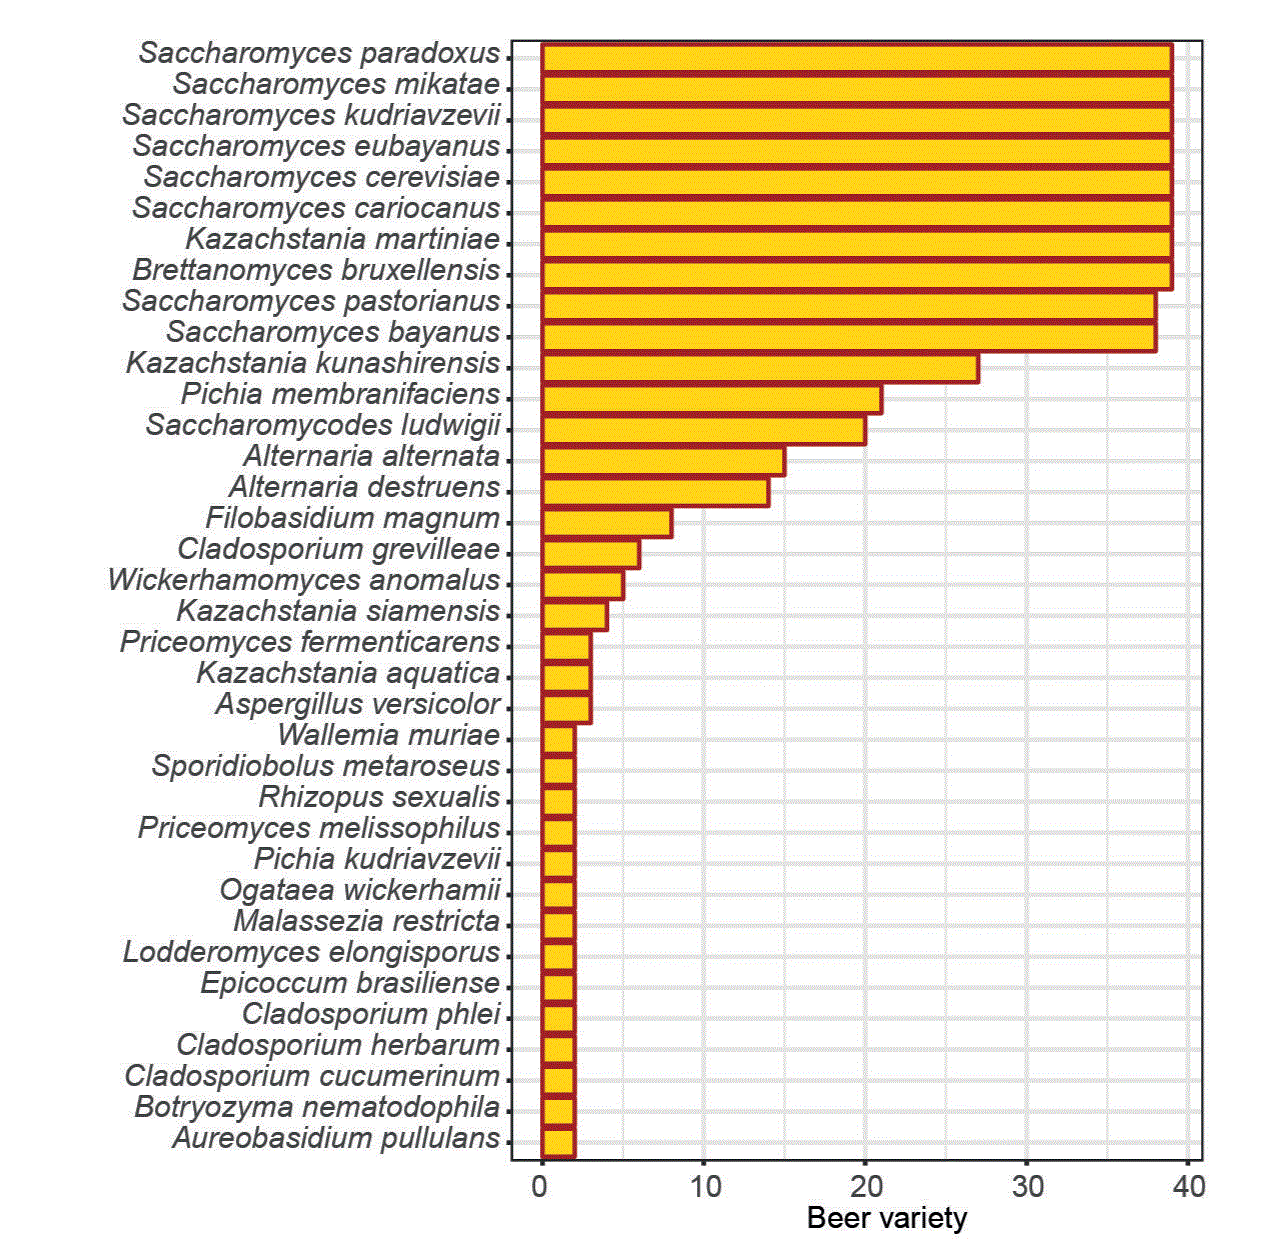
\includegraphics[width=\textwidth]{images/orginal_BeerDEcoded_beer_variety.png}
        \caption{Orginal result}
        \label{fig:results:orginal_BeerDecoded_beer_variety}
    \end{subfigure}
    \hfill
    \begin{subfigure}[b]{0.45\textwidth}
        \centering
        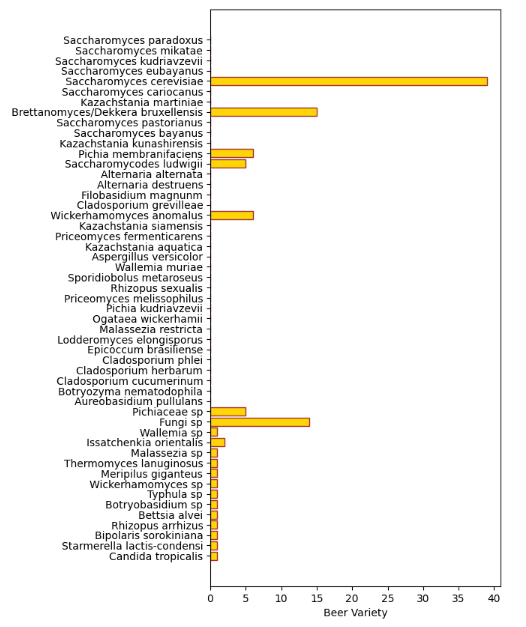
\includegraphics[width=\textwidth]{images/BeerDEcoded_beer_variety.png} 
        \caption{Reproduced results}
        \label{fig:results:reproduced_BeerDecoded_beer_variety}
    \end{subfigure}
    \caption{BeerDecoded beer variety diagram}
    \small The figures present data regarding the quantity of beers associated with each species identified in both the original and reproduced results. For clarity, the figure depicting the reproduced results on the right retains the species order as presented in the original figure. This arrangement aids in a more transparent comparison between the two sets of results.
    \label{fig:results:BeerDecoded_beer_variety}
\end{figure}


    Upon examining the heatmap \ref{fig:results:BeerDecoded_heatmap}, we observe, as expected, that \textit{Saccharomyces} is the most prevalent species, identified in every beer sample, a finding that is in line with the broader BeerDEcoded project results. The next most common species is \textit{Brettanomyces bruxellensis}, appearing in 15 samples, a species found in all samples within the BeerDEcoded project. Unexpectedly, an organism labeled as \textit{Fungi sp} is also found in high abundance. Further investigation revealed that \textit{Fungi sp} is labeled as 'unidentified' in the database. At present, we are uncertain whether this status is due to the workflow's inability to accurately identify it as a known species, or if it truly remains unclassified in the database.

    \begin{figure}[H]
        \centering
        \begin{subfigure}[b]{0.6\textwidth}
            \centering
            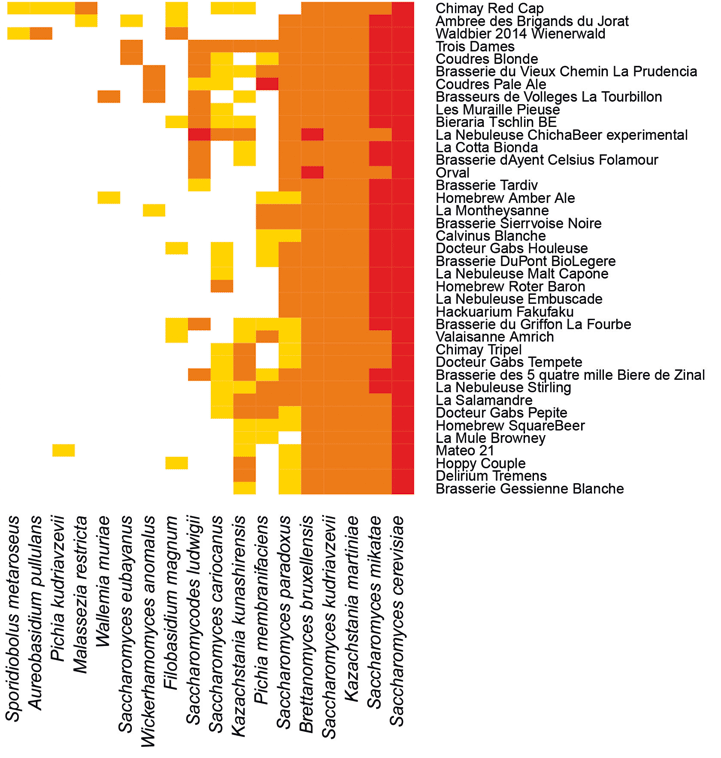
\includegraphics[width=\textwidth]{images/beerdecoded/orginal_beerDecoded_heatmap.png}
            \caption{Original results}
            \label{fig:results:oringal_BeerDecoded_heatmap}
        \end{subfigure}
        \hfill
        \begin{subfigure}[b]{0.6\textwidth}
            \centering
            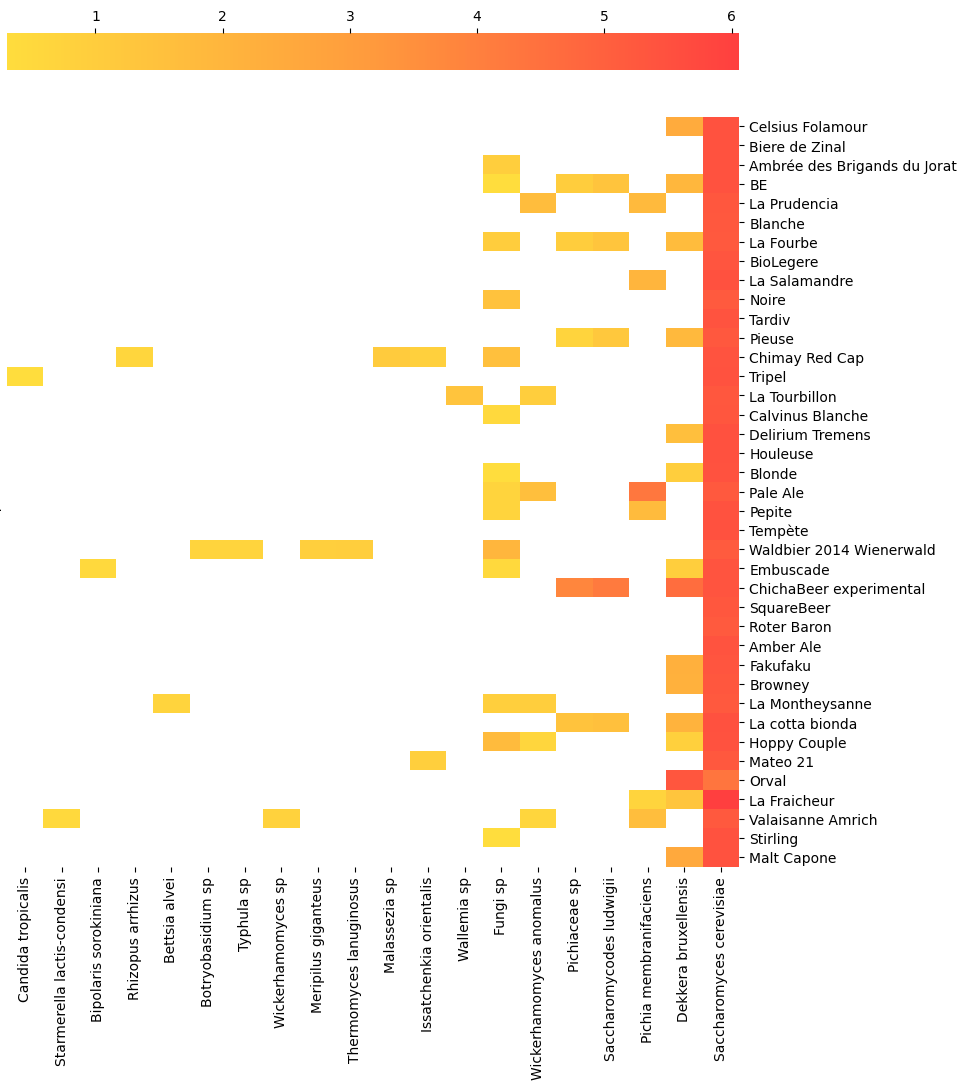
\includegraphics[width=\textwidth]{images/beerdecoded/BeerDecoded_heatmap.png}
            \caption{Reproduced results}
            \label{fig:results:reproduced_BeerDecoded_heatmap}
        \end{subfigure}
        \caption{Heatmap of the number of reads per ITS per beer}
        \small Beer names are shown on the right and species names are shown at the bottom.
        \label{fig:results:BeerDecoded_heatmap}
    \end{figure}
    
    In contrast to the BeerDecoded project, our analytic process was unable to detect 31 species that were identified in the BeerDecoded study. However, we did discover 7 species not previously identified. This discrepancy could potentially stem from the relatively low quality of the samples, which averaged a quality score of around 20. As we utilized the QIIME 2 and BLAST consensus methodologies for taxonomy classification, the less-than-ideal quality could lead to ambiguous results. In instances where one feature sequence may be linked to more than two species, it could result in the feature being labeled as unidentified. This classification approach is notably different from the strategy adopted in the BeerDecoded study. In the latter, they followed an unconventional methodology of constructing a database with assumed taxonomies presumed to be present in the samples. They then proceeded to map the sequences directly to their custom-built database.

\subsubsection{Bacterial and Fungal Dynamics During the Fermentation Process of Sesotho, a Traditional Beer of Southern Africa}

    % \begin{figure}[H]
    %     \centering
    %     \includegraphics[scale=0.7]{images/sesotho_species_relative_abundance.png}
    %     \caption{Sesotho species relative abundance}
    %     \label{fig:methods:sesotho_species_relative_abundance}
    % \end{figure}


     The collection of Sesotho samples took place from five different districts (breweries) namely, Maseru (MSU), Mafeteng (MFT), Thaba-Tseka (HN), Butha-Buthe (Butha), and Mokhotlong (MK). Within each location, five samples were obtained, representing various stages of fermentation. The first sample (1) was gathered one hour after the initial starter culture was added to commence the first fermentation phase. Subsequently, the second sample (2) was obtained at approximately eight hours into the fermentation process, after the completion of the first fermentation phase. The third sample (3) was collected one hour after introducing the second starter culture, which initiated the second and final fermentation phase. Following that, the fourth sample (4) was acquired approximately eight hours after the second fermentation, prior to the beer undergoing sieving, which involves the separation of sorghum malt from the beer. Lastly, the fifth sample (5) was taken from the final product, around eight hours into the maturation stage.
    
    Figures \ref{fig:results:sesotho_phyla_relative_abundance}, \ref{fig:results:sesotho_family_relative_abundance}, and \ref{fig:results:sesotho_genus_relative_abundance}, presented in this thesis and the original study, respectively, depict the distribution of fungal taxa in Sesotho beer at the Phylum, Family, and Genus levels.

    \begin{figure}[H]
        \centering
        \begin{subfigure}[b]{1\textwidth}
            \centering
            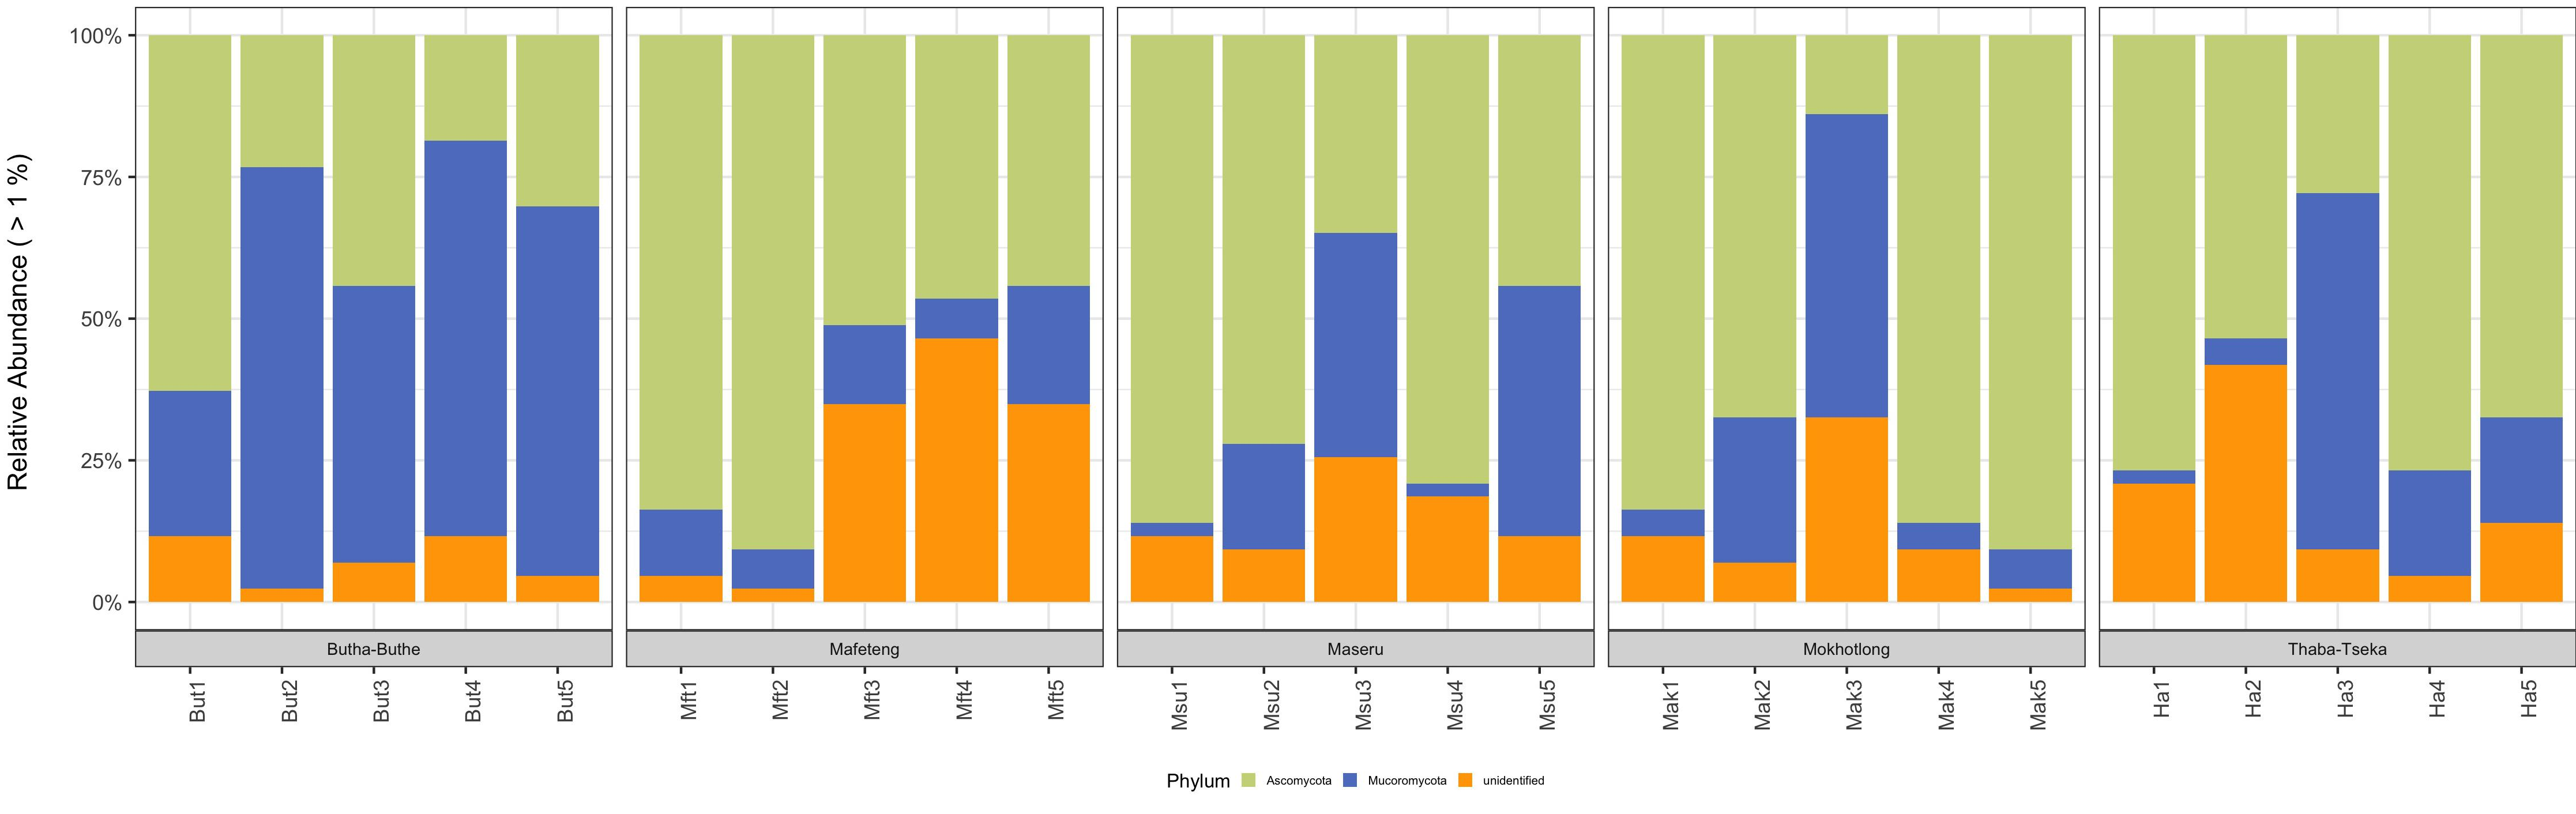
\includegraphics[width=\textwidth]{images/sesotho/original_sesotho_phyla_relative_abundance.png}
            \caption{Original results}
            \label{fig:results:original_sesotho_phyla_relative_abundance}
        \end{subfigure}
        \hfill
        \begin{subfigure}[b]{1\textwidth}
            \centering
            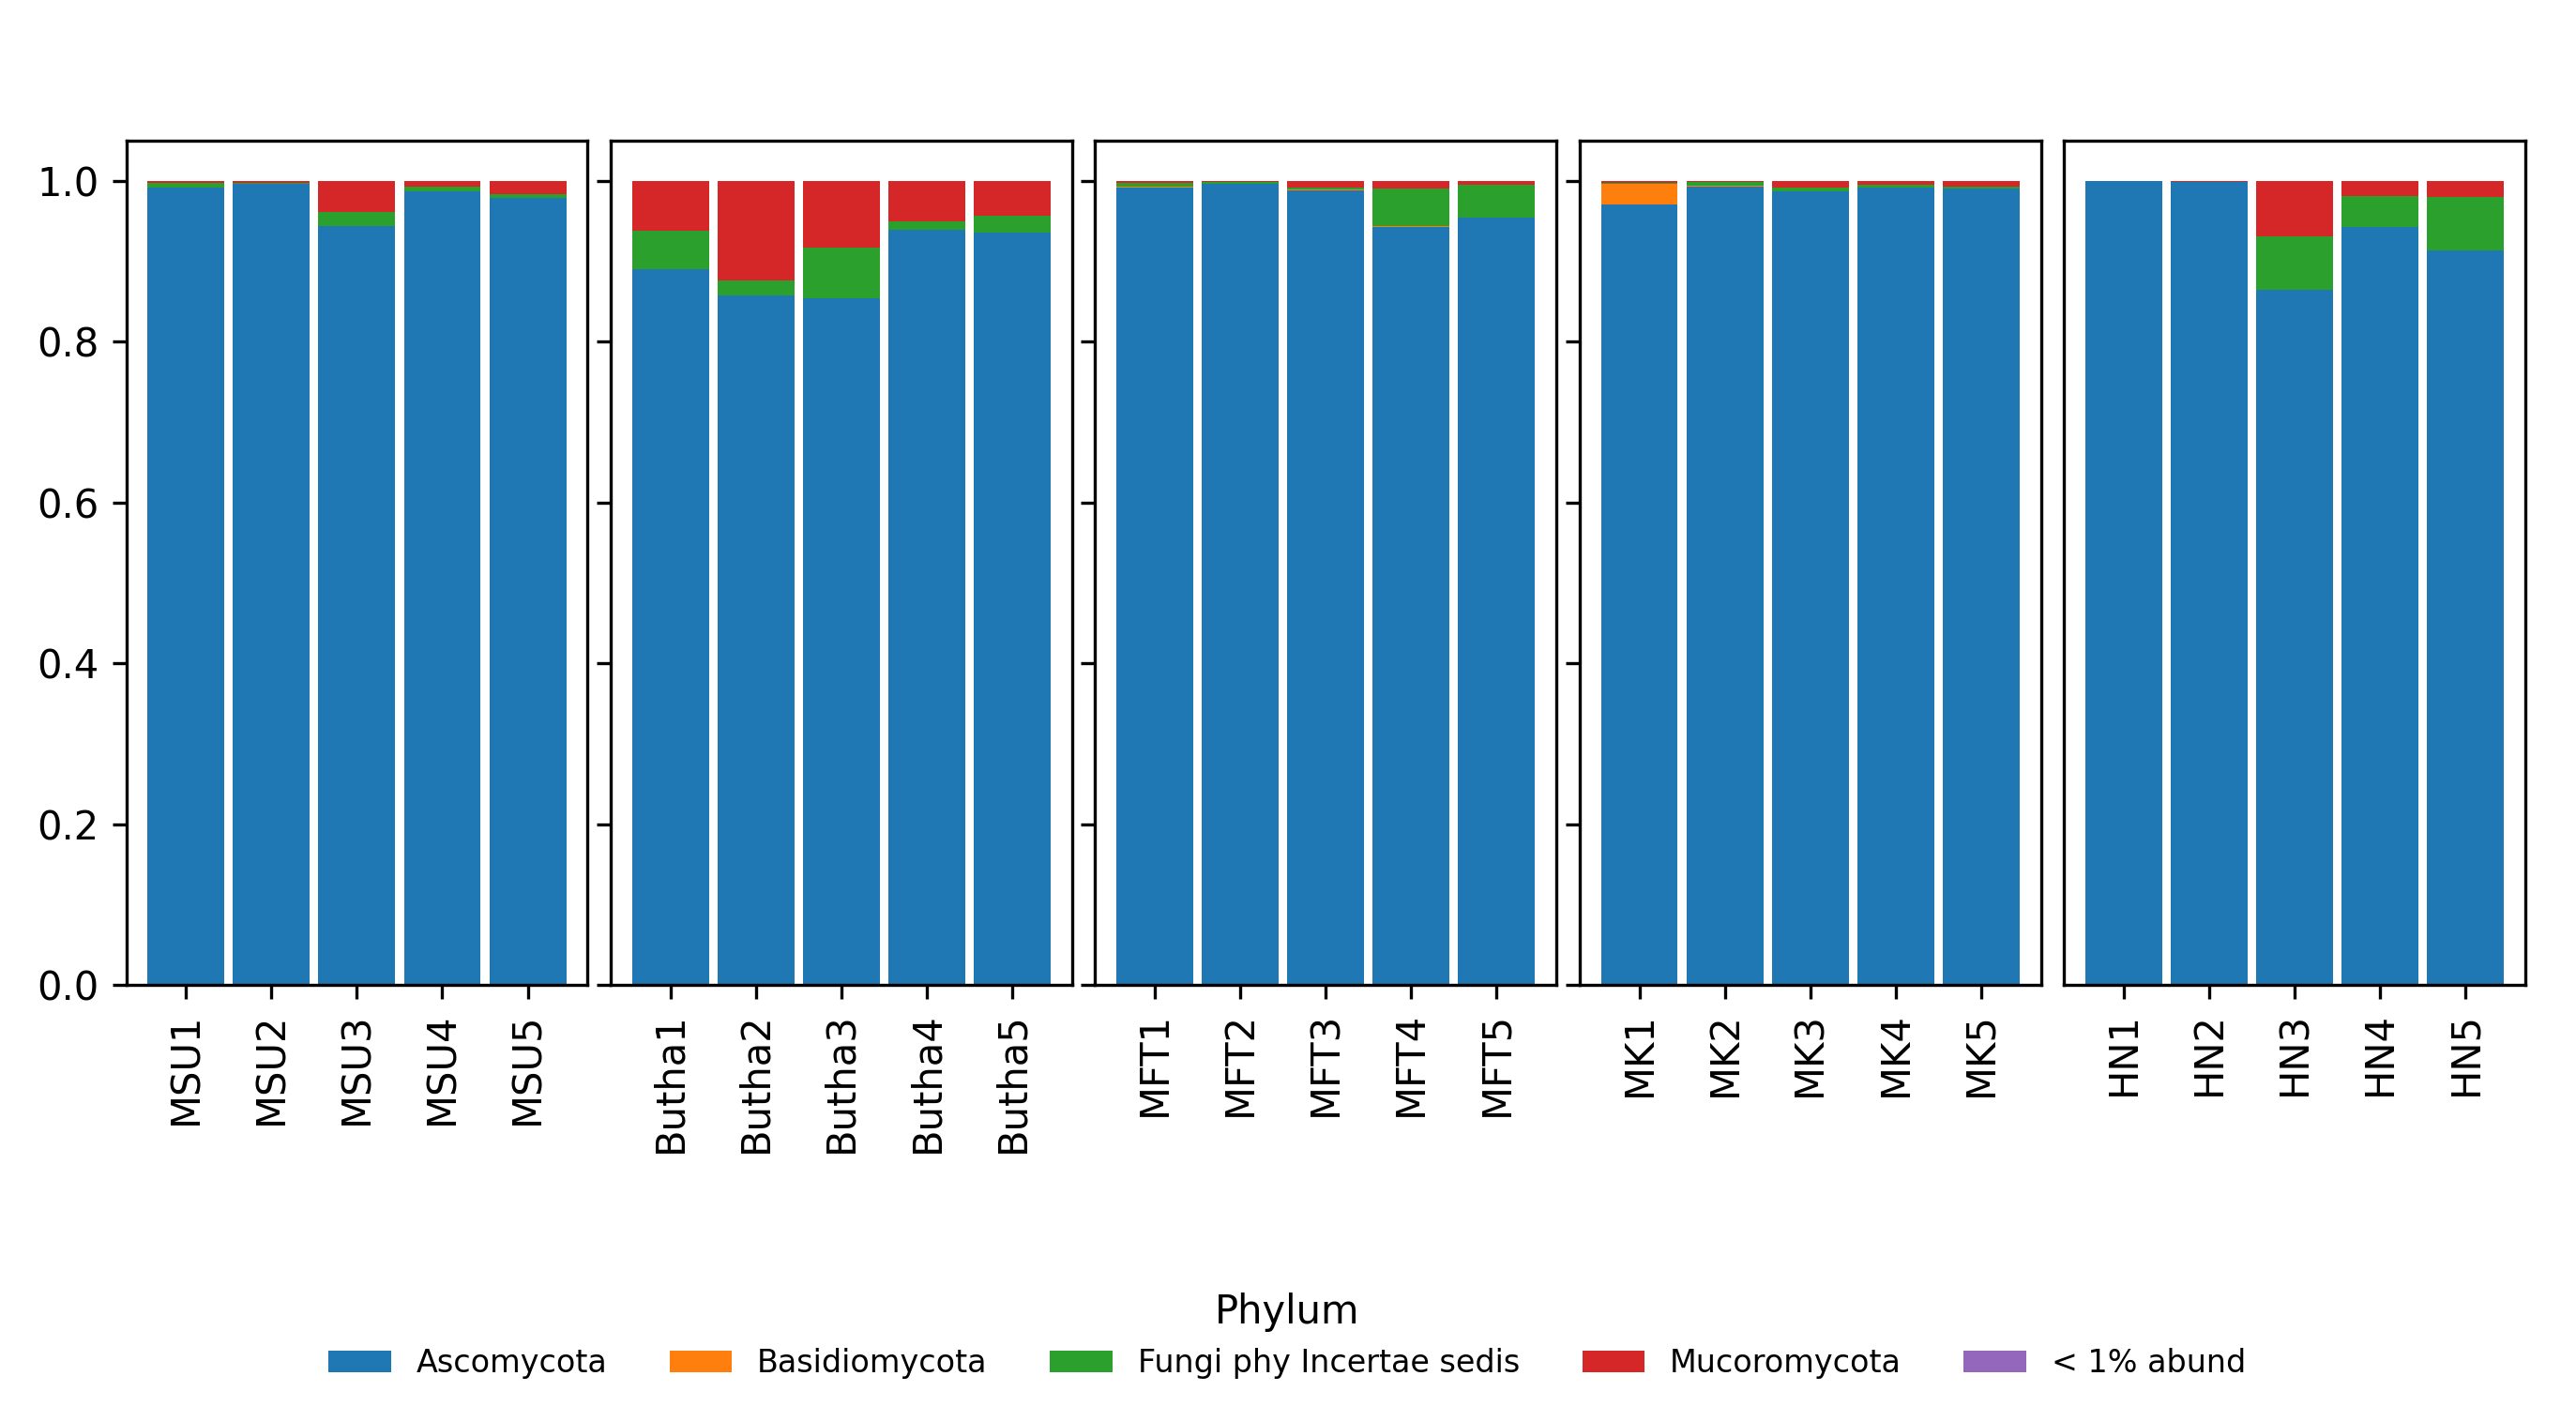
\includegraphics[width=\textwidth]{images/sesotho/sesotho_phyla_relative_abundance.png}
            \caption{Reproduced results}
            \label{fig:results:reproduced_sesotho_phyla_relative_abundance}
        \end{subfigure}
        \caption{Distribution of fungal Phylum in Sesotho.}
        \small In the graphical representation, the x-axis delineates the various breweries, labeled as Maseru (MSU), Mafeteng (MFT), Thaba-Tseka (HN), Butha-Buthe (Butha), and Mokhotlong (MK). To illustrate, the label "MK1" denotes a sample sourced from Mokhotlong during the first stage of fermentation. The fungal phyla Ascomycota and Mucoromycota emerged as the predominant groups in the study. Notably, Ascomycota displayed a higher dominance in the reproduced results compared to the original findings.
        \label{fig:results:sesotho_phyla_relative_abundance}
    \end{figure}
    
    Similar to the original findings, Ascomycota and Mucoromycota were the predominant fungal phyla observed in all samples and locations as shown in figure \ref{fig:results:sesotho_phyla_relative_abundance}. However, in this thesis, the presence of Basidiomycota was also identified. Basidiomycota fungi are widely distributed in nature and can be found in various habitats such as soil, plants, and air. If the raw ingredients, such as sorghum or maize, are contaminated with Basidiomycota spores during the brewing process, these spores can enter the beer mixture and subsequently proliferate during fermentation.

        \begin{figure}[H]
        \centering
        \begin{subfigure}[b]{1\textwidth}
            \centering
            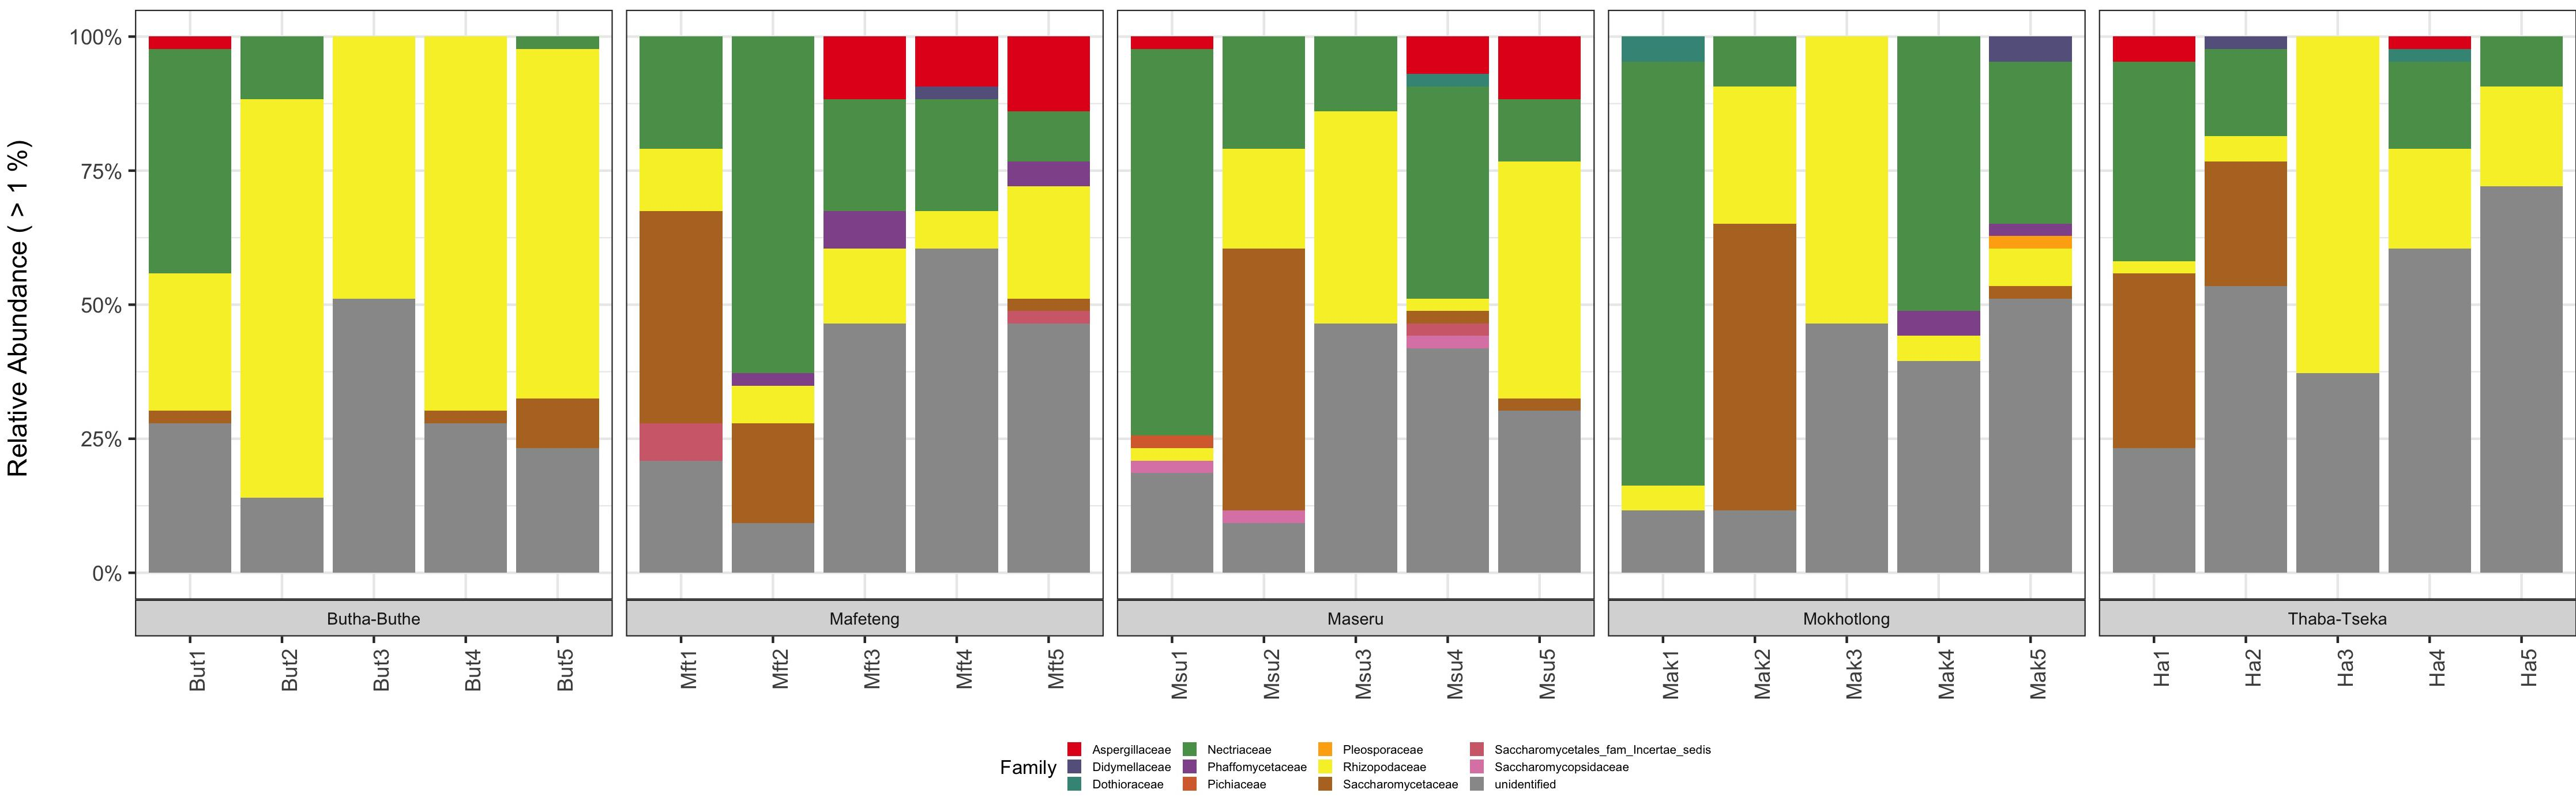
\includegraphics[width=\textwidth]{images/sesotho/original_sesotho_families_relative_abundance.png}
            \caption{Original results}
        \end{subfigure}
        \hfill
        \begin{subfigure}[b]{1\textwidth}
            \centering
            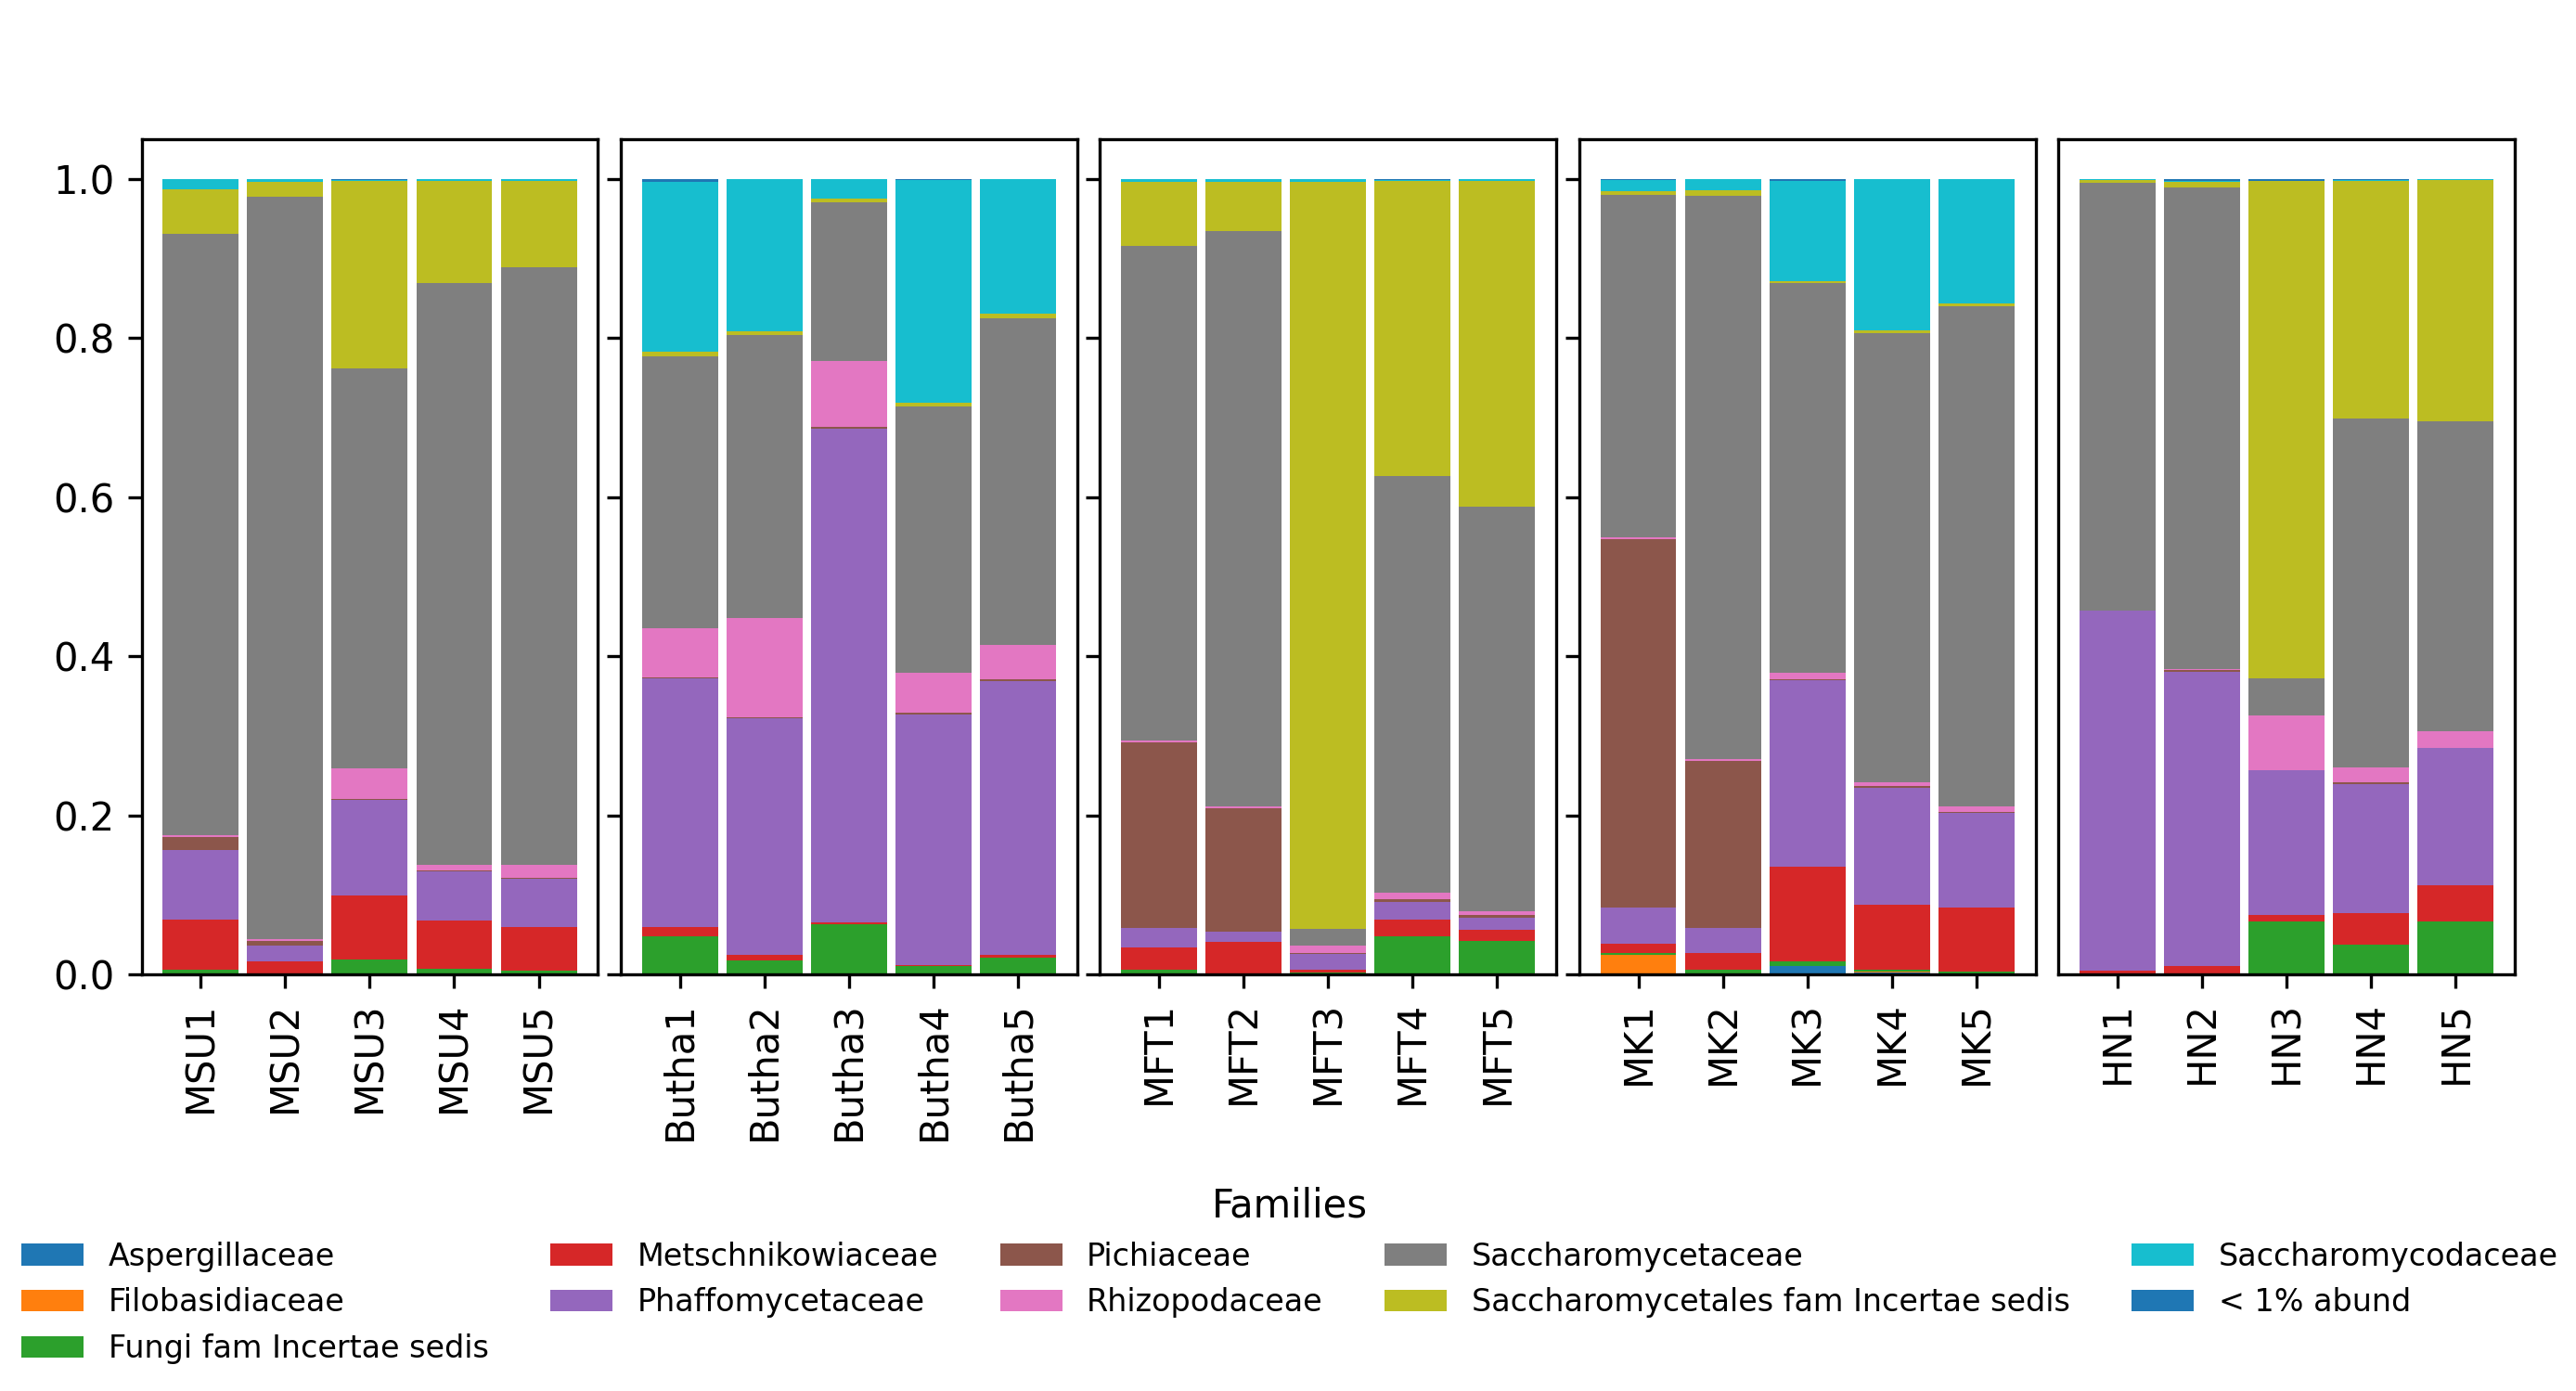
\includegraphics[width=\textwidth]{images/sesotho/sesotho_family_relative_abundance.png}
            \caption{Reproduced results}
        \end{subfigure}
        \caption{Distribution of fungal Family in Sesotho.}
        \small In alignment with the original findings, the reproduced data also identified the presence of \textit{Phaffomycetaceae} and \textit{Pichiaceae}.
        \label{fig:results:sesotho_family_relative_abundance}
    \end{figure}
    
    As seen in figure \ref{fig:results:sesotho_family_relative_abundance}, consistent with the Original results, we observed the presence of \textit{Saccharomycetaceae} and \textit{Nectriaceae} from the Phylum Ascomycota, as well as \textit{Rhizopodaceae} from the Phylum Mucoromycota. Additionally, we detected a substantial abundance of \textit{Phaffomycetaceae} and \textit{Pichiaceae}, which are families of yeasts belonging to the order Saccharomycetales.

    \begin{figure}[H]
        \centering
        \begin{subfigure}[b]{1\textwidth}
            \centering
            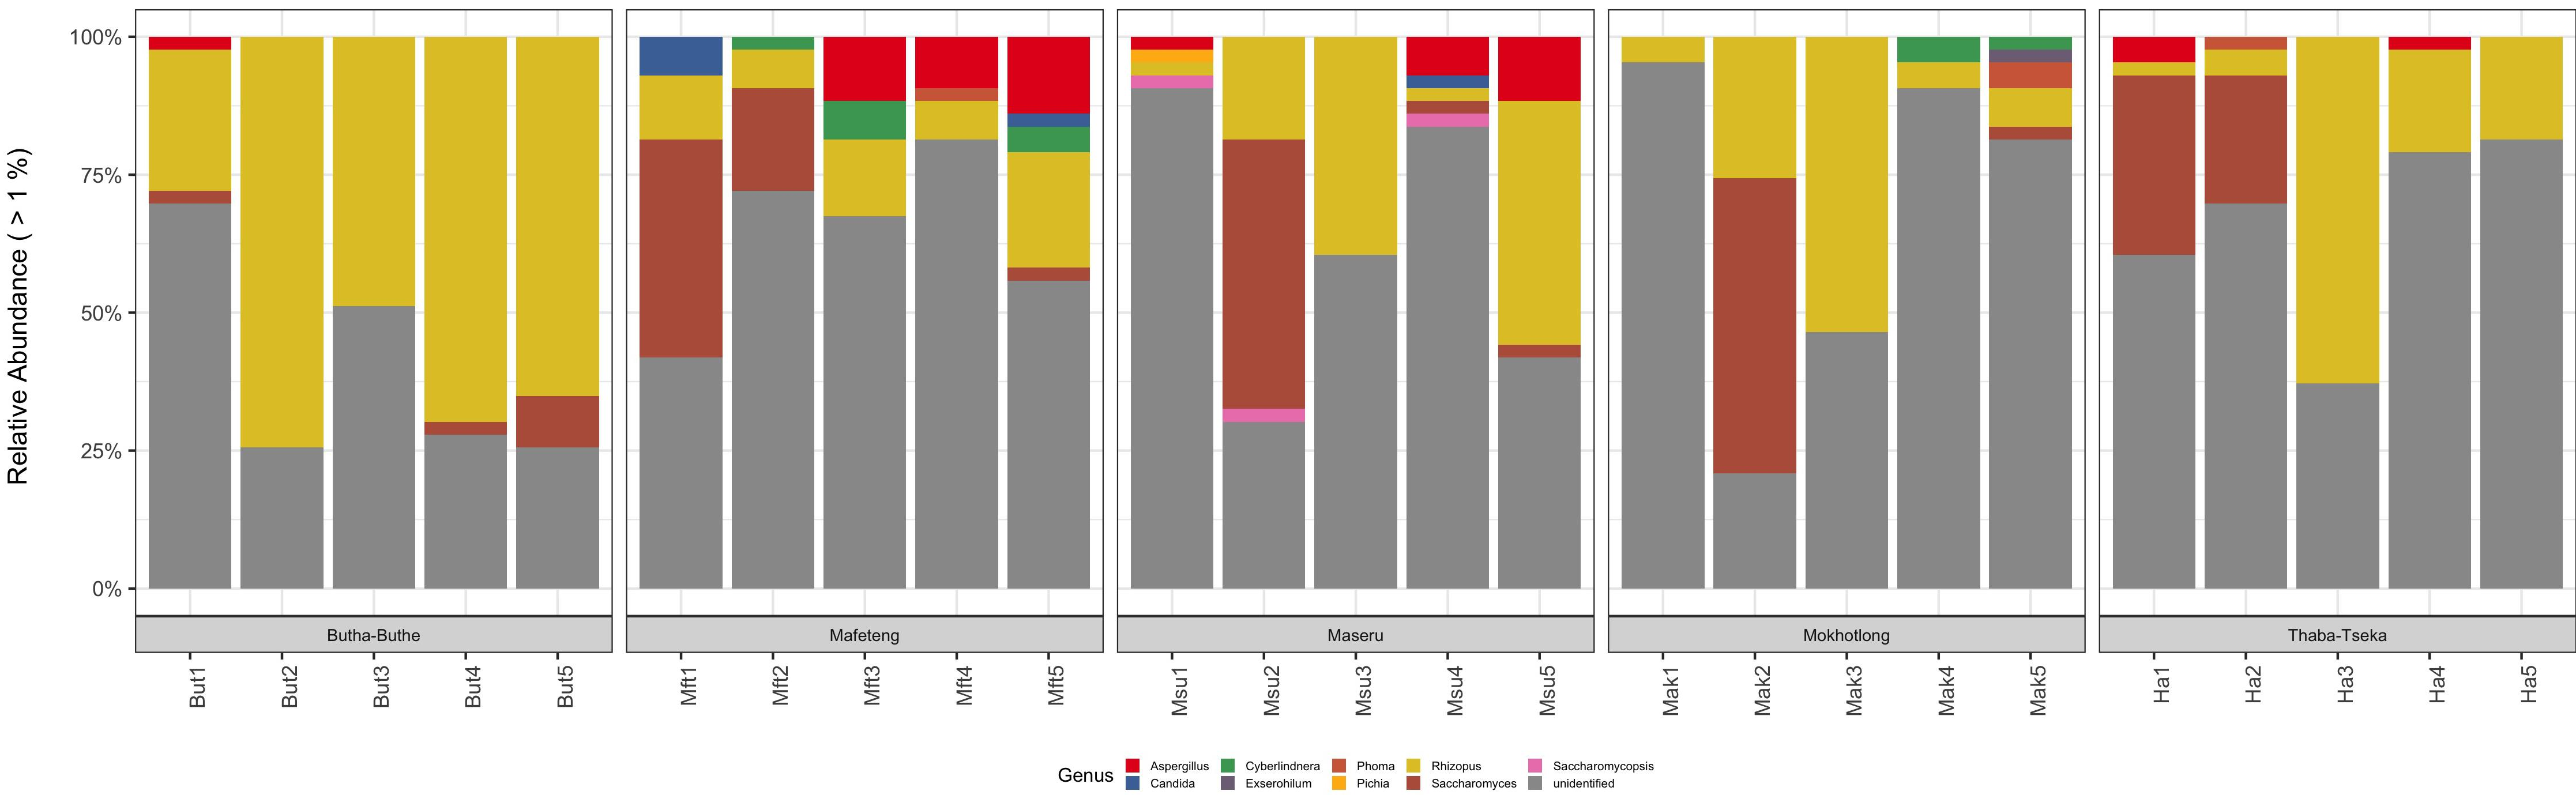
\includegraphics[width=\textwidth]{images/sesotho/original_sesotho_genera_relative_abundance.png}
            \caption{Original results}
        \end{subfigure}
        \hfill
        \begin{subfigure}[b]{1\textwidth}
            \centering
            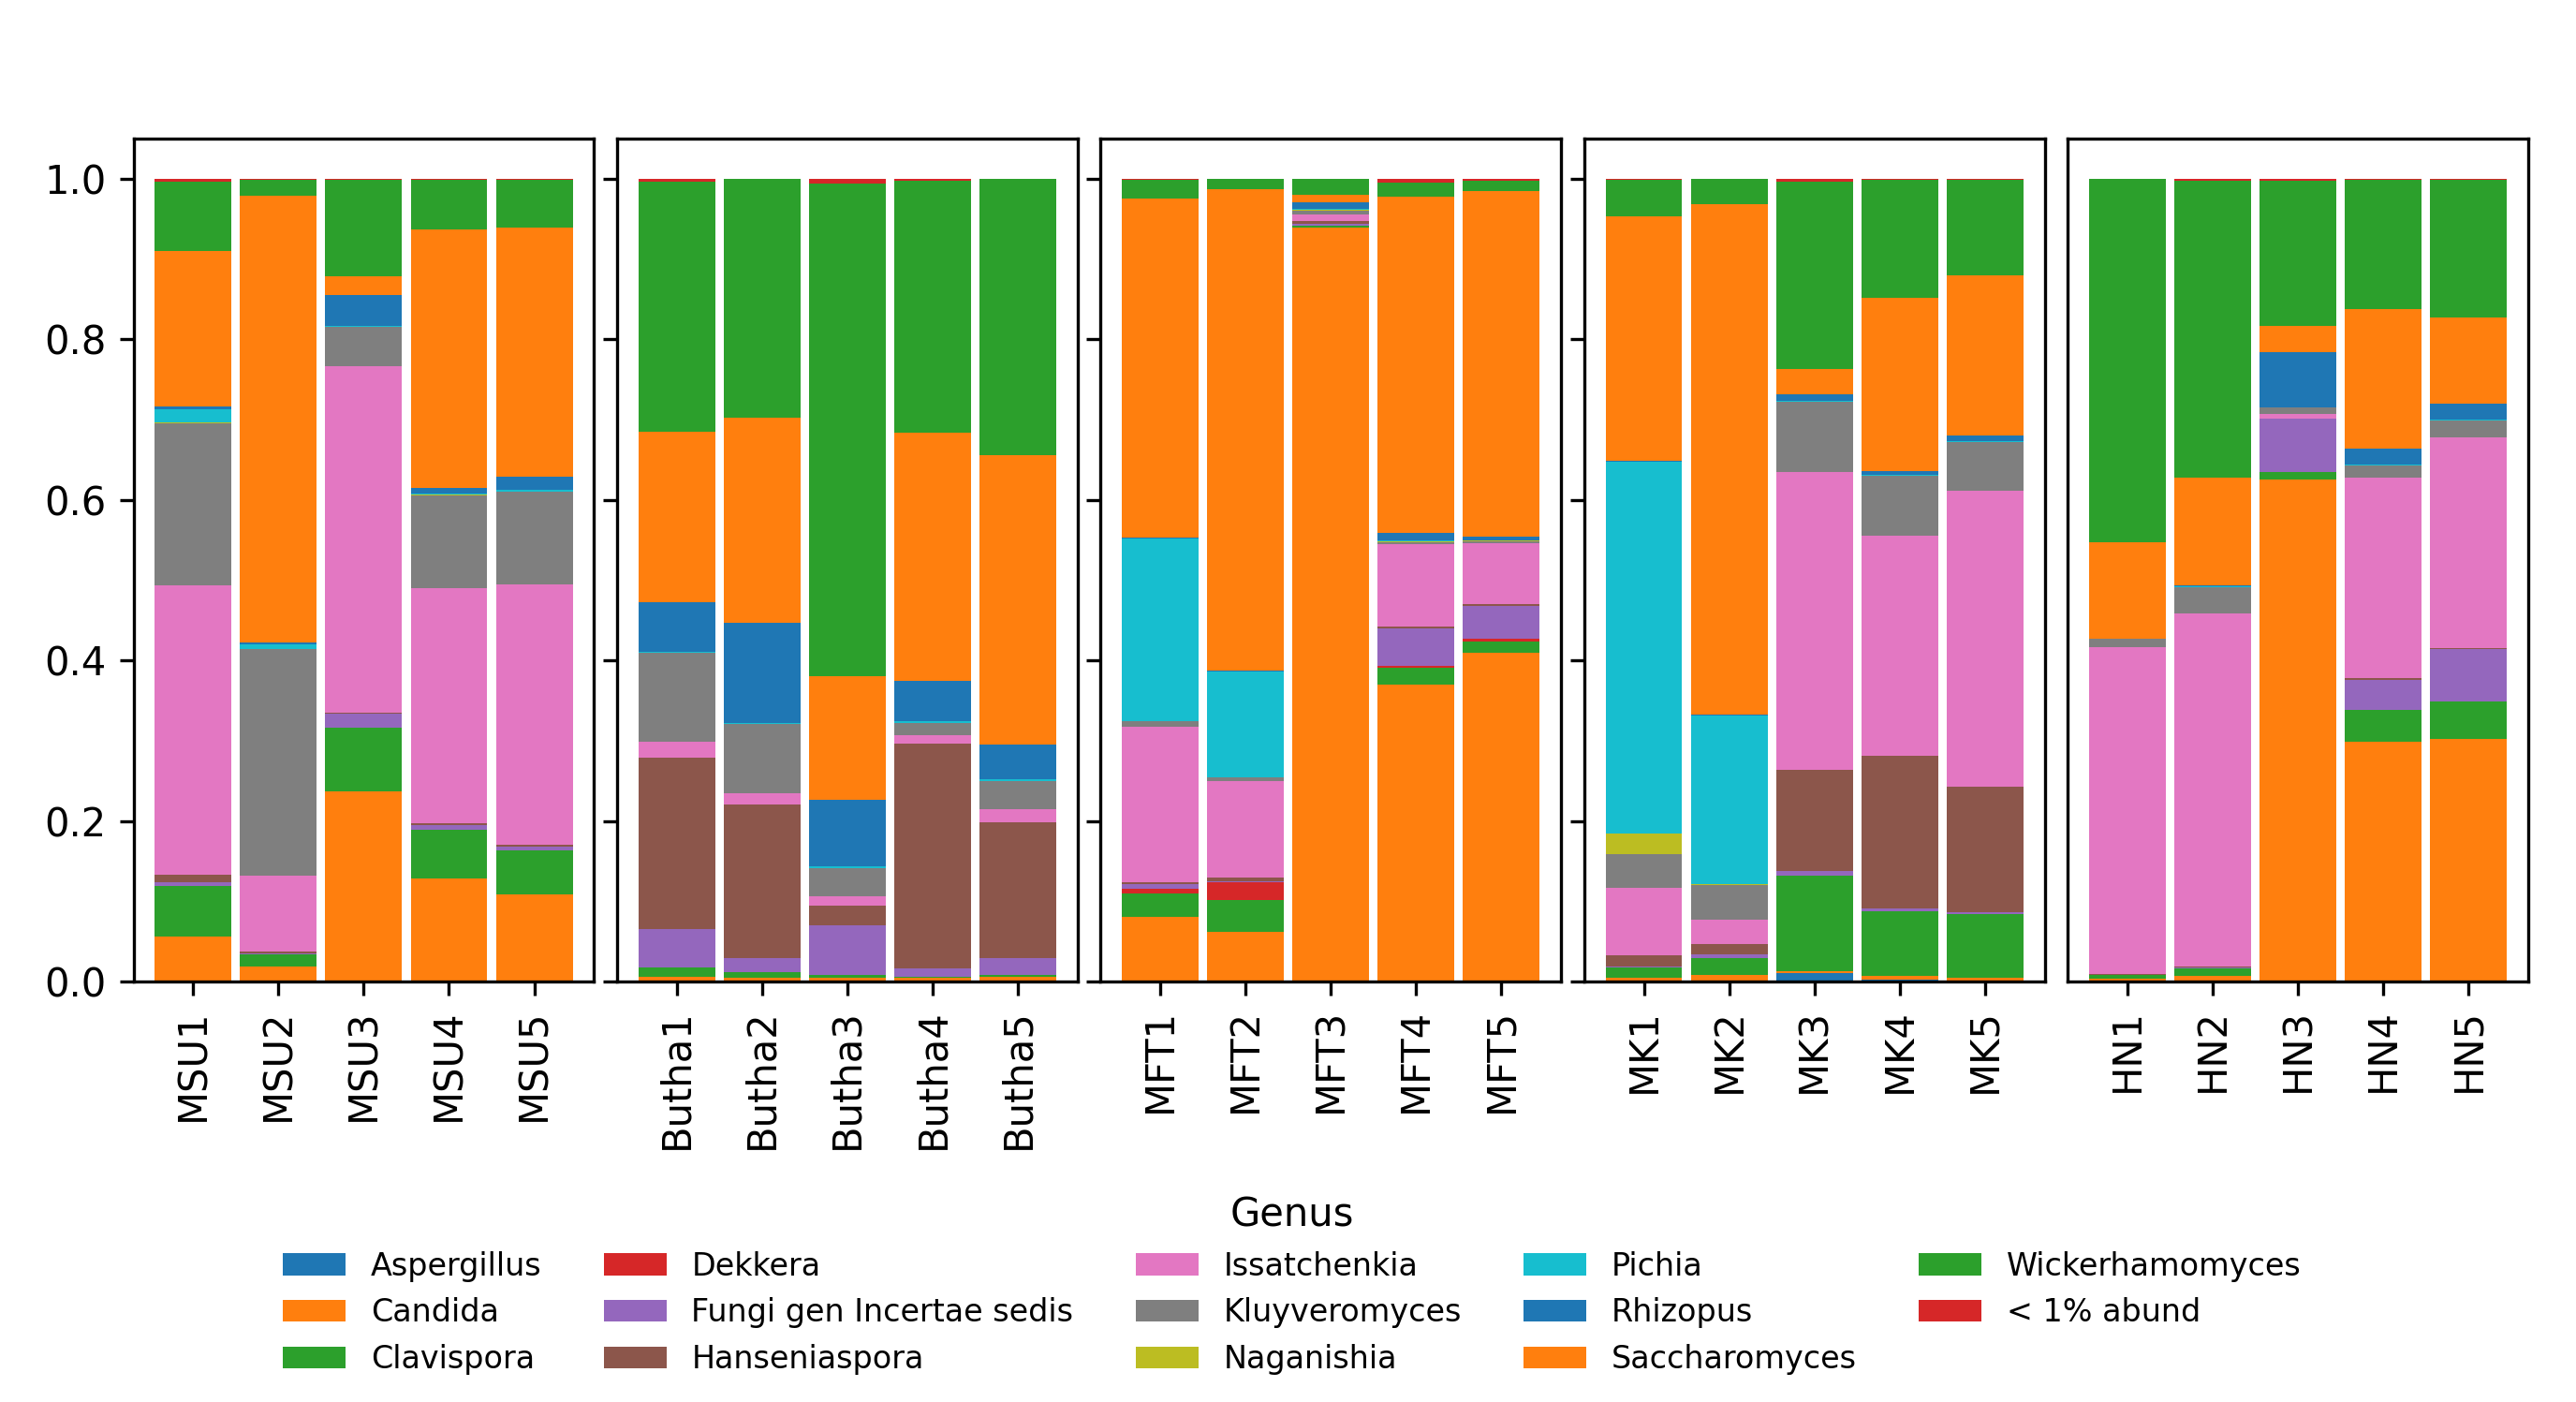
\includegraphics[width=\textwidth]{images/sesotho/sesotho_genus_relative_abundance.png}
            \caption{Reproduced results}
        \end{subfigure}
        \caption{Distribution of fungal Genus in Sesotho}
        \small Based on the analysis of the distribution of fungal genera in Sesotho, \textit{Rhizopus} emerges as the dominant genus in the original findings. In contrast, \textit{Saccharomyces} is more prevalent in the reproduced data.
        \label{fig:results:sesotho_genus_relative_abundance}
    \end{figure}
    
    Unlike the original findings, where \textit{Saccharomyces} was most prevalent in the 1st and 2nd stages of the brewing process, our analysis revealed the presence of \textit{Saccharomyces} throughout all stages of brewing (Figure \ref{fig:results:sesotho_genus_relative_abundance}). Moreover, \textit{Wickerhamomyces} was also found in significant abundance, which is a genus of fungi within the \textit{Saccharomycetales} order. \textit{Wickerhamomyces anomalus} is known to produce a faintly pleasant odor.

    Overall, this thesis demonstrates a greater diversity of fungal taxa at all taxonomic levels compared to the original study. This disparity could be attributed to the utilization of QIIME 2 instead of QIIME 1, as well as the incorporation of an updated version of the UNITE database, which likely contributed to enhanced taxonomic resolution and accuracy in our analysis.
    
\subsubsection{A Culture-Independent Comparison of Microbial Communities of Two Maturating Craft Beers Styles}

    For this study, two beer styles produced by a commercial craft brewery were selected. The first beer style, named Extra, is classified as a Doppelbock Lager and has an alcohol content of 8\%. The second beer style, called Rubi, falls under the category of a Märzen Lager and has an alcohol content of 6.3\%.

    \paragraph*{Fungal diversity}
    Contrary to other studies shown above, the analysis revealed that \textit{Saccharomyces} was not the dominant genus in spontaneously-fermented craft beer, consistent with previous findings\cite{shayevitz2020barrel}. Instead, the most abundant genus in both beer styles was \textit{Dekkera}, represented by the species \textit{D. bruxellensis}, \textit{D. anomala}, and \textit{D. custersiana} (Figure \ref{fig:methods:doppelbock_relative_abundence_fungal}). This suggests that a souring process occurs during maturation, contributing to the flavor profile. Additionally, \textit{Zygosaccharomyces}, known for its association with fruity flavors \cite{methner2019screening}, was also detected in the reproduced result, consistent with the original findings.
    
\begin{figure}[H]
    \centering
    \begin{subfigure}[b]{0.45\textwidth}
        \centering
        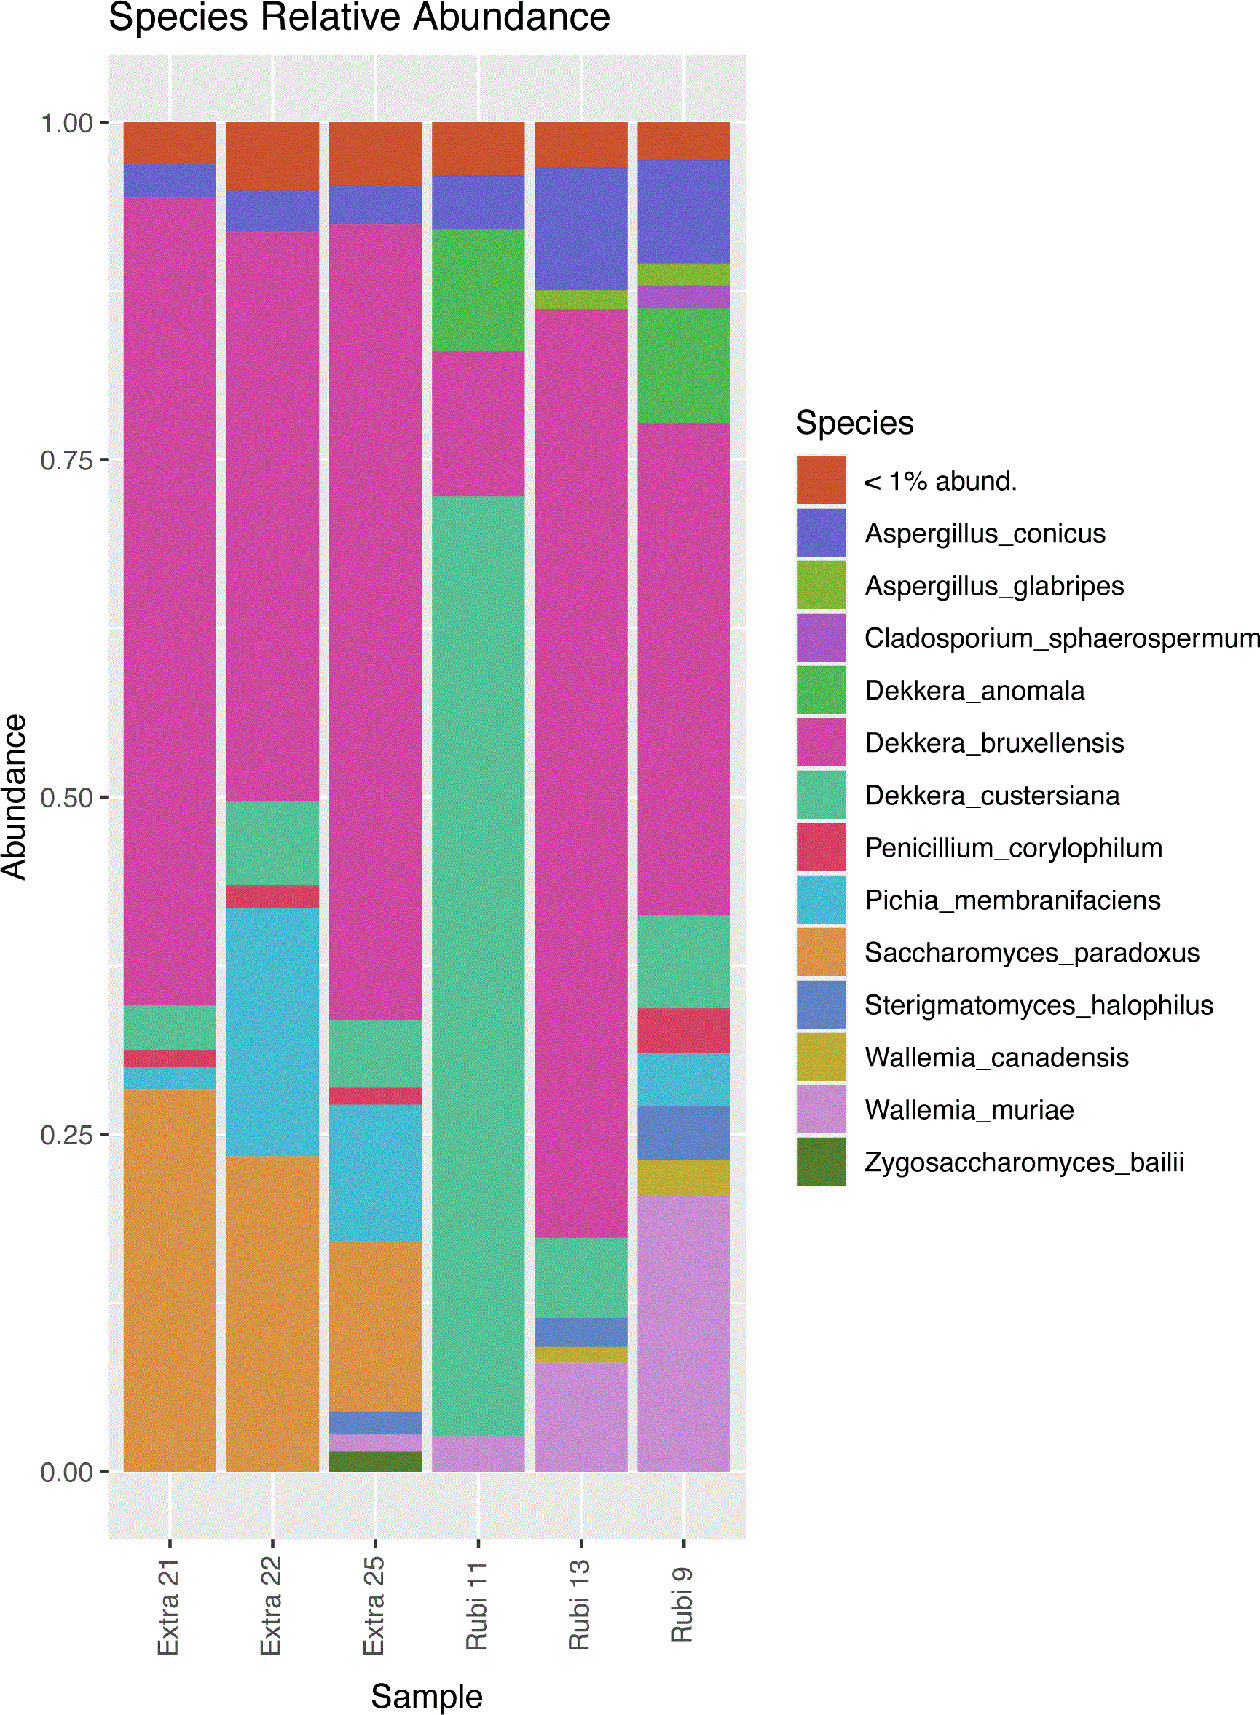
\includegraphics[width=\textwidth]{images/orginal_doppelbock_relative_abundence.jpg}
        \caption{Original results}
    \end{subfigure}
    \hfill
    \begin{subfigure}[b]{0.45\textwidth}
        \centering
        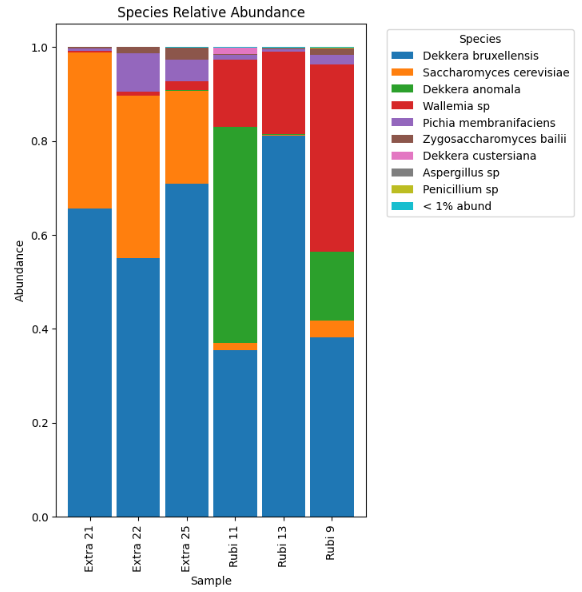
\includegraphics[width=\textwidth]{images/doppelbock_relative_abundence.png}
        \caption{Reproduced results}
    \end{subfigure}
    \caption{Fungal species relative abundance}
    \small The relative abundance of fungal taxa at the species level across various beer styles is depicted. Notably, \textit{Dekkera} stands out as the most abundant genus in both beer styles examined.
    \label{fig:methods:doppelbock_relative_abundence_fungal}
\end{figure}

    In addition to the presence of \textit{Pichia}, the Original results showed the detection of \textit{Aspergillus} and \textit{Penicillium}. Notably, \textit{Hanseniaspora uvarum}, a yeast commonly found on grapes\cite{fleet1993wine}, was also identified, indicating its presence in the samples.

    
\begin{table}[H]
\centering
\begin{threeparttable}
\caption{Comparison of Original and reproduced estimates and T-test results}
\begin{tabular}{c}
\begin{subtable}{\textwidth}
\centering
\caption{Species richness and diversity of fungal communities in Extra and Rubi beer barrels}
\begin{tabular}{|c|c|c|c|c|c|c|}
\hline
\multirow{2}{*}{Sample} & \multicolumn{2}{c|}{Chao1} & \multicolumn{2}{c|}{Shannon} & \multicolumn{2}{c|}{Simpson} \\ \cline{2-7} 
                        & Original & Reproduced & Original & Reproduced & Original & Reproduced \\ \hline
Extra \#21              & 48    & 42  & 2.07    & 2.50    & 0.83    & 0.76    \\ \hline
Extra \#22              & 67.5  & 61  & 2.45    & 2.94    & 0.87    & 0.80    \\ \hline
Extra \#25              & 98.6  & 94  & 2.53    & 3.31    & 0.86    & 0.82    \\ \hline
Rubi \#11               & 70.5  & 65  & 1.88    & 3.46    & 0.72    & 0.82    \\ \hline
Rubi \#13               & 90.2  & 89  & 2.16    & 2.71    & 0.77    & 0.65    \\ \hline
Rubi \#9                & 117.2 & 104 & 3.14    & 4.16    & 0.92    & 0.89    \\ \hline
\end{tabular}
\end{subtable}
\\
\begin{subtable}{\textwidth}
\centering
\caption{T-test results for Original vs Reproduced estimates}
\begin{tabular}{|l|r|r|}
\hline
  Index &  T-statistic &  p-value \\
\hline
  Chao1 &    -3.238 & 0.0230 \\
\hline
Shannon &    -8.748 & 0.0003 \\
\hline
Simpson &     7.000 & 0.0009 \\
\hline
\end{tabular}
\end{subtable}
\end{tabular}
\begin{tablenotes}[flushleft]
\footnotesize
\item \textbf{Note:} Chao1 represents the Chao1 species richness estimator.
\item Shannon denotes the Shannon index of biodiversity. Higher values indicate higher diversity.
\item Simpson represents the Simpson diversity index. Values range from 0 (simplest) to 1 (most diverse).
\end{tablenotes}
\end{threeparttable}
\label{tab:combined_table}
\end{table}

Upon reviewing the results from the original study and the reproduced results of diversity indices for the beer samples on the diversity of fungal communities, several notable points of comparison and contrast emerge.

First, looking at the Chao1 biodiversity index, the reproduced results indicate generally lower estimates across all samples, with a noticeable decrease in Rubi \#9 (from 117.2 to 104) and Extra \#21 (from 48 to 42). Chao1 is a non-parametric estimator used to predict the true species richness of a community, and thus these lower estimates suggest that the reproduced results predict fewer unique species in each sample than the original study.

In contrast, the Shannon index, which measures the entropy (or unpredictability) of species diversity within a community, is consistently higher in the reproduced results across all samples. This suggests that the reproduced results found a greater degree of diversity, possibly with more evenly distributed species within each sample. The most pronounced differences can be observed in Rubi \#11 (from 1.88 to 3.46) and Extra \#22 (from 2.45 to 2.94).

Similarly, the Simpson index, which is a measure of species diversity that gives more weight to the abundant species, also shows an increase in all but one sample (Rubi \#13, where it decreased from 0.77 to 0.65) in the reproduced results. This suggests an increased evenness and diversity, as a higher Simpson's index implies that individuals are distributed more evenly among species.

In summary, with these differences in individual measures and t-test results, the data suggests that the reproduced results have more evenly distributed diversity but less richness.

    \paragraph*{Bacterial diversity}

In our reanalysis of the bacterial communities present in two distinct styles of beer, we found the overall bacterial distribution to be consistent with the original study (Figure \ref{fig:methods:doppelbock_relative_abundence_bacterial}). The primary microbial constituents encompassed just three genera, each with a relative abundance of 1\% or more. These pivotal genera were identified as \textit{Pediococcus}, \textit{Lactobacillus}, and \textit{Acetobacter}.

\begin{figure}[H]
     \centering
     \begin{subfigure}[b]{0.45\textwidth}
         \centering
         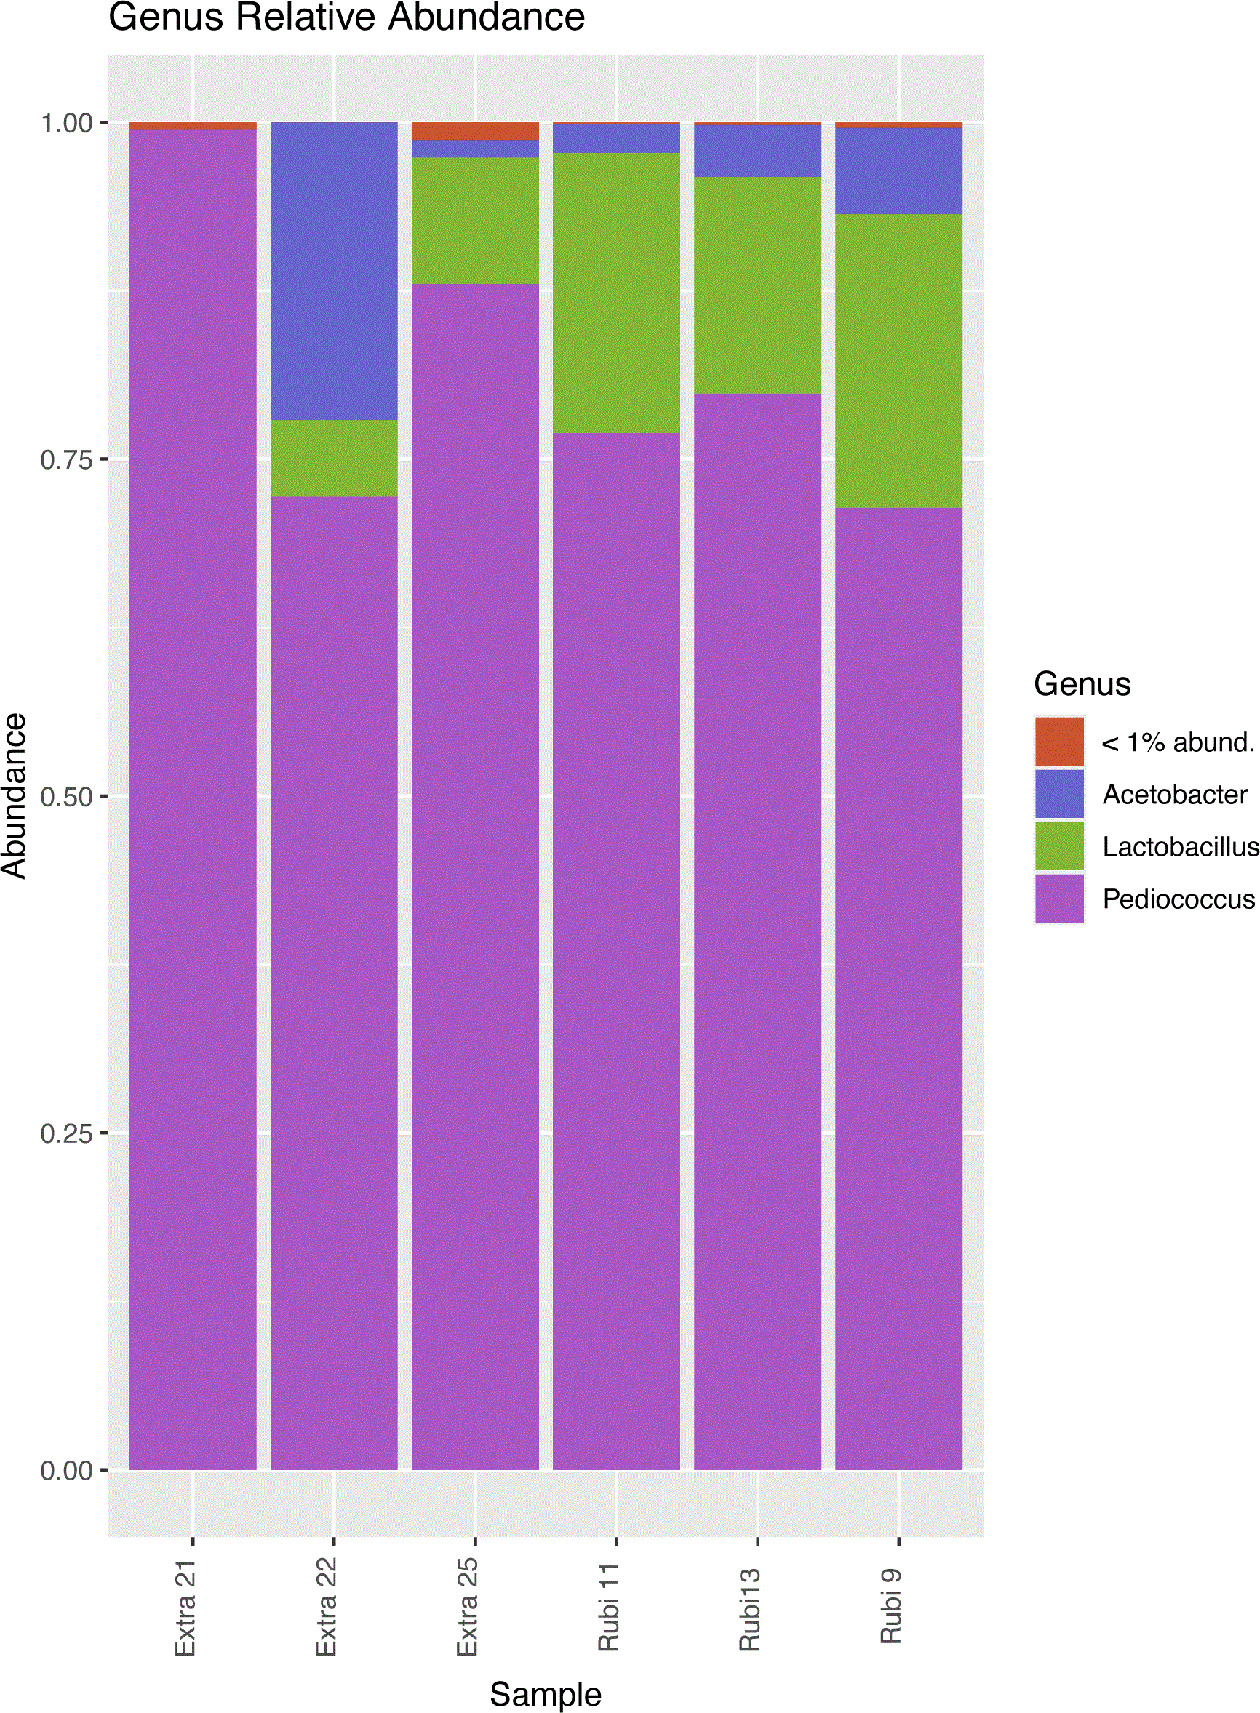
\includegraphics[width=\textwidth]{images/original_doppel_baceteria_genus_relative_abundance.jpg}
        \caption{Original results}
     \end{subfigure}
     \hfill
     \begin{subfigure}[b]{0.45\textwidth}
         \centering
         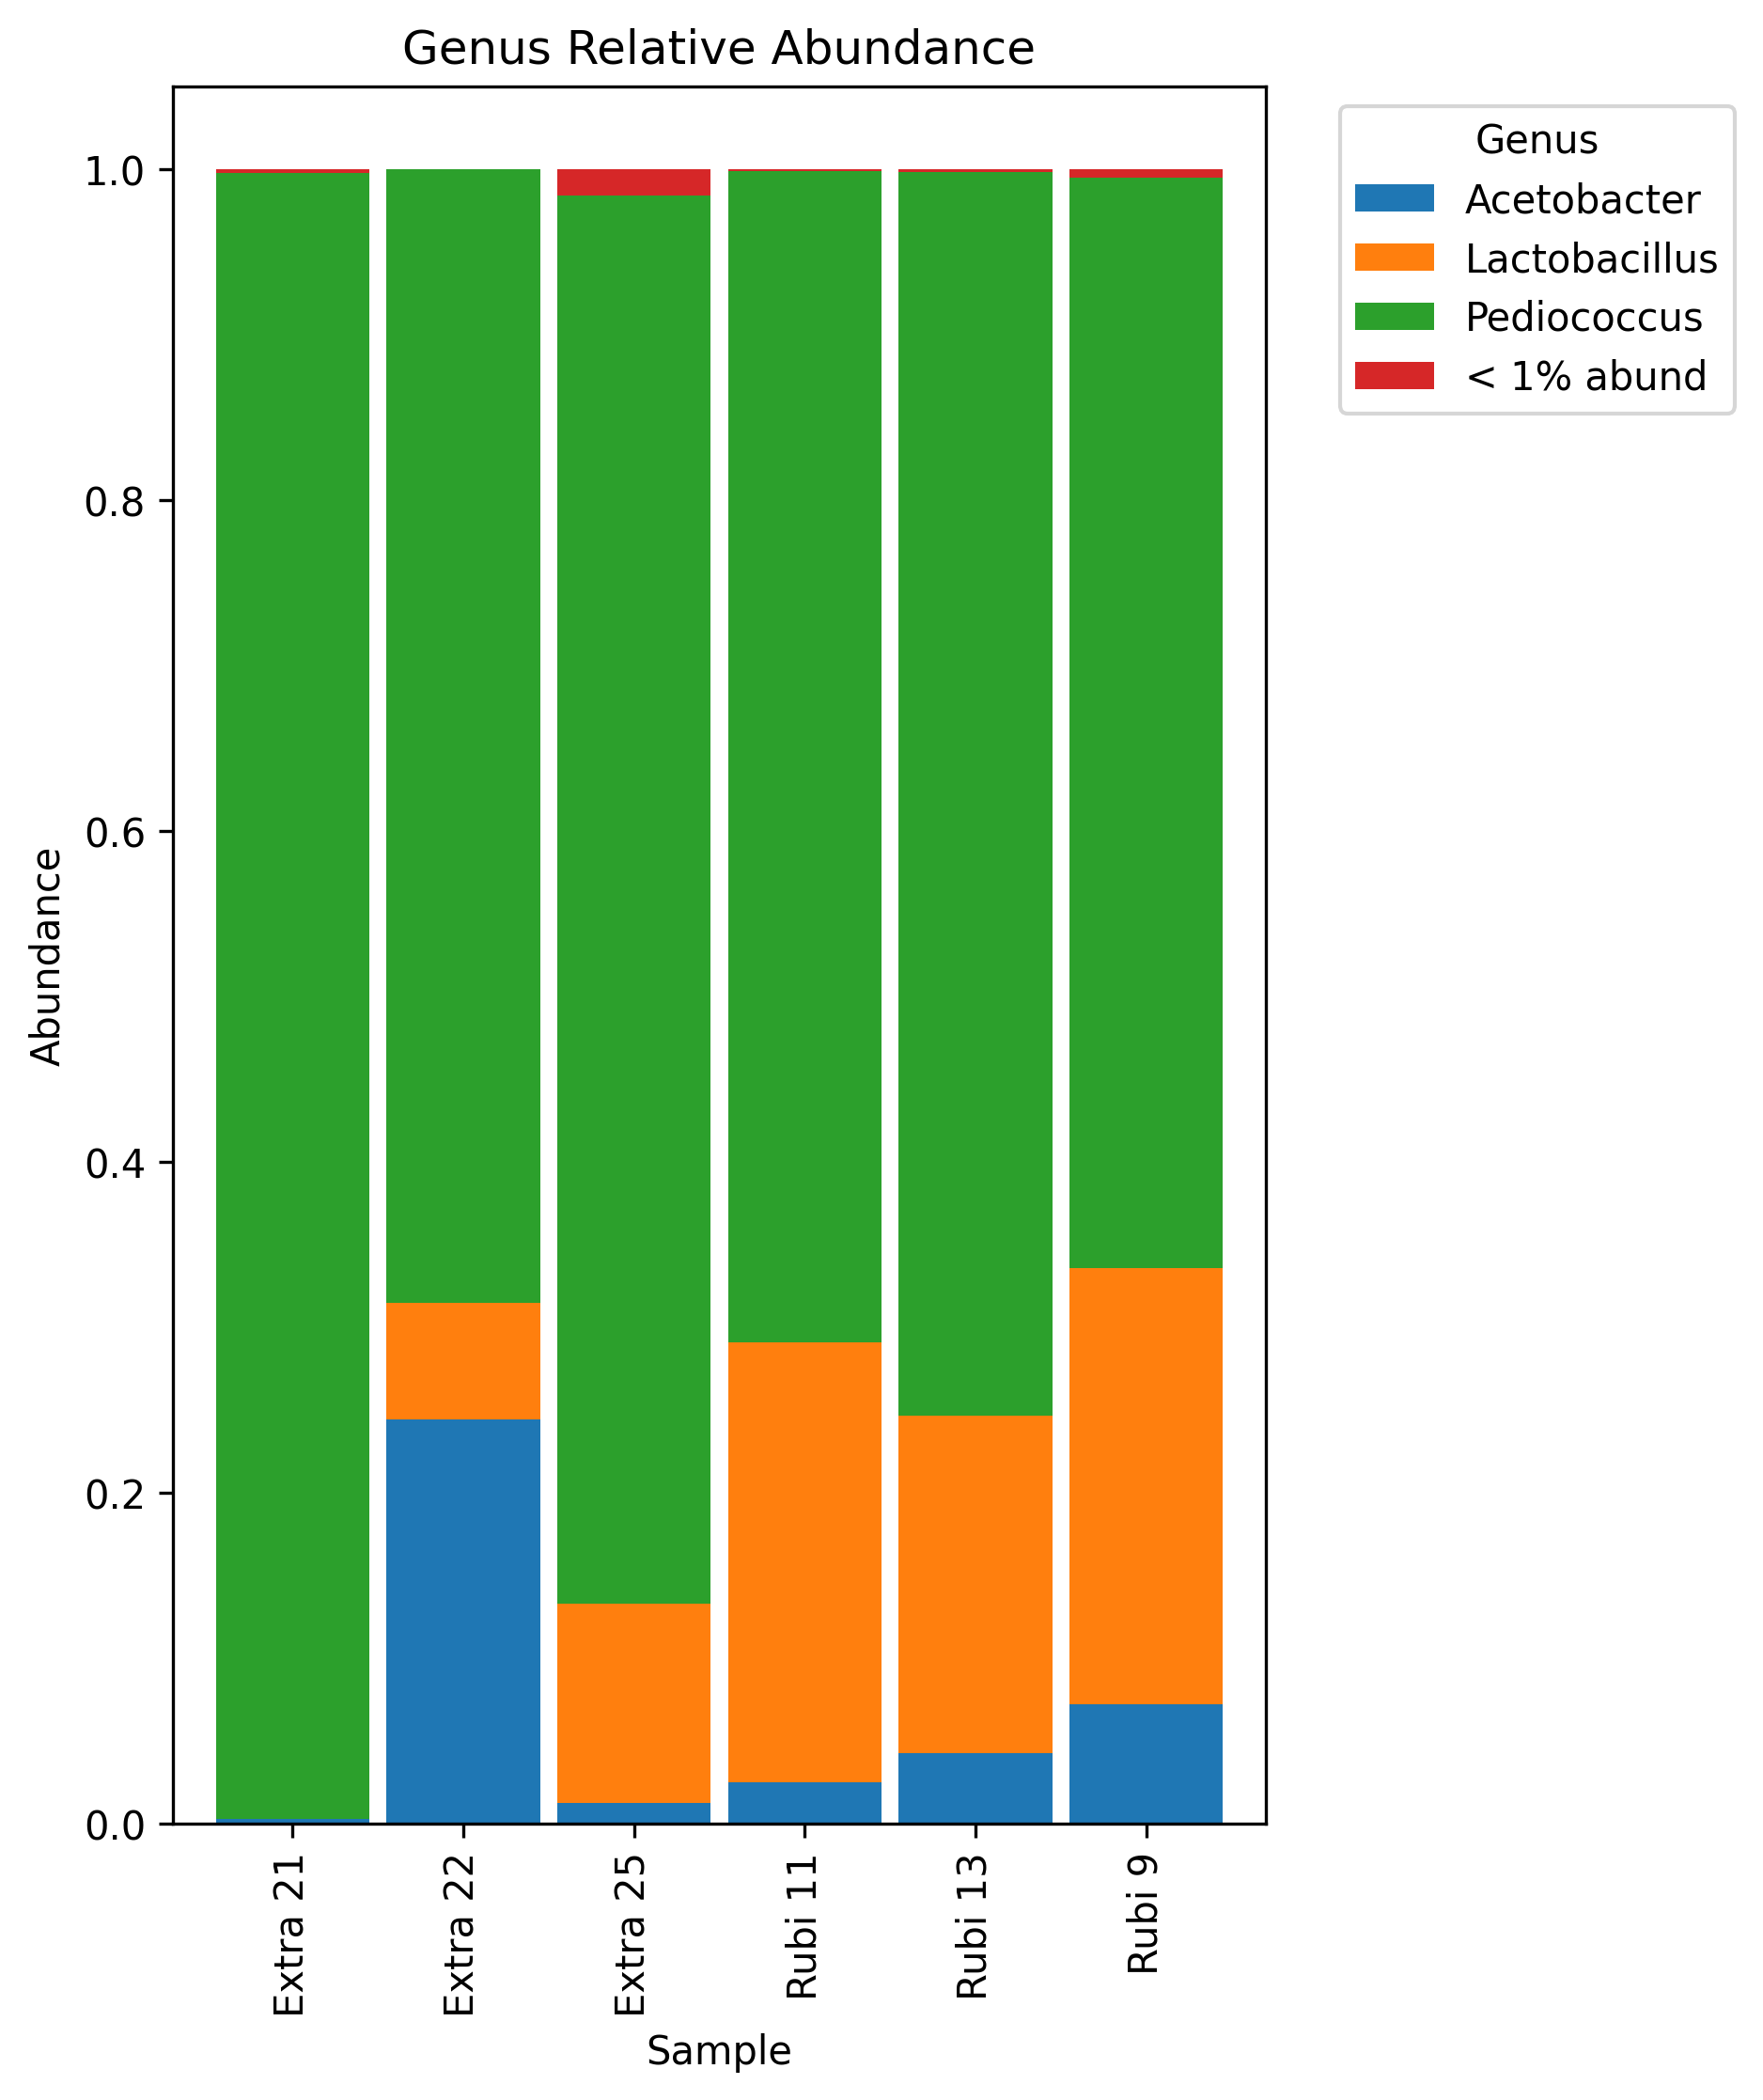
\includegraphics[width=\textwidth]{images/doppel_baceteria_genus_relative_abundance.png}
        \caption{Reproduced results}
     \end{subfigure}
    \caption{Bacterial genus relative abundance}
    \small Regarding the relative abundance of bacterial taxa at the genus level within the beer styles, the produced results align well with the findings of the original study.
    \label{fig:methods:doppelbock_relative_abundence_bacterial}
\end{figure}

Discrepancies in the prevalence of these bacterial genera were more pronounced in the samples of Extra beer when compared to the Ruby variant. A stark example was found in Extra barrel \#21 where \textit{Pediococcus} appeared to be the predominant microorganism, accounting for a staggering 99\% of the bacterial population. Conversely, Extra barrel \#22 was characterized by the highest percentage of \textit{Acetobacter} across all beer samples, recorded at 22\%. Extra barrel \#25 was notable for exhibiting the greatest abundance of \textit{Lactobacillus} among the Extra samples. Interestingly, this marked variability was not reflected in the Ruby beer samples. Instead, we observed a much more uniform distribution of bacterial genera across the Ruby barrels.


\begin{table}[h!]
\centering
\begin{threeparttable}
\caption{Comparison of Original and reproduced estimates and T-test results}
\begin{tabular}{c}
\begin{subtable}{\textwidth}
\centering
\caption{Species richness and diversity of bacterial communities in Extra and Rubi beer barrels}
\begin{tabular}{|c|c|c|c|c|c|c|}
\hline
\multirow{2}{*}{Sample} & \multicolumn{2}{c|}{Chao1} & \multicolumn{2}{c|}{Shannon} & \multicolumn{2}{c|}{Simpson} \\ \cline{2-7} 
                        & Original & Reproduced & Original & Reproduced & Original & Reproduced \\ \hline
Extra \#21              & 10   & 13  & 1.45    & 1.73    & 0.74    & 0.66    \\ \hline
Extra \#22              & 10   & 13  & 1.86    & 2.45    & 0.82    & 0.78    \\ \hline
Extra \#25              & 18   & 31  & 1.88    & 2.57    & 0.81    & 0.77    \\ \hline
Rubi \#11               & 9    & 19  & 1.72    & 2.27    & 0.80    & 0.76    \\ \hline
Rubi \#13               & 17   & 24  & 1.96    & 2.69    & 0.83    & 0.79    \\ \hline
Rubi \#9                & 10   & 11  & 1.75    & 2.30    & 0.81    & 0.77    \\ \hline
\end{tabular}
\end{subtable}
\\
\begin{subtable}{1\textwidth}
\centering
\caption{T-test results for Original vs reproduced estimates}
\begin{tabular}{|l|r|r|}
\hline
  Index &  T-statistic &  p-value \\
\hline
  Chao1 &     3.845 & 0.012 \\
\hline
Shannon &    -4.537 & 0.006 \\
\hline
Simpson &     1.257 & 0.264 \\
\hline
\end{tabular}
\end{subtable}
\end{tabular}
\begin{tablenotes}[flushleft]
\footnotesize
\item \textbf{Note:} Chao1 represents the Chao1 species richness estimator.
\item Shannon denotes the Shannon index of biodiversity. Higher values indicate higher diversity.
\item Simpson represents the Simpson diversity index. Values range from 0 (simplest) to 1 (most diverse).
\end{tablenotes}
\end{threeparttable}
\label{tab:combined_table}
\end{table}


The Chao1 index, an estimator of species richness, appears to show higher values in the reproduced results than in the original, for all samples. The increase in Chao1 values implies that the re-analysis might have identified more species within the samples. A T-test comparing the original and reproduced Chao1 values reveals a significant difference with a p-value of 0.012. This indicates that the difference in species richness estimates between the original and reproduced data is not likely due to chance.

For the Shannon index, which incorporates both species richness and evenness, the reproduced results also display higher values for all samples. The T-test further corroborates this observation with a statistically significant p-value of 0.006. Higher Shannon values suggest that the bacterial communities identified in the re-analysis are not only richer in species but also display a more even distribution among the identified species.

In contrast, the Simpson index, which places greater weight on dominant species, reveals no statistically significant difference between the original and reproduced estimates (p-value = 0.264). This suggests that, despite variations in species richness and evenness, the overall dominance structure of the bacterial communities remains relatively consistent between the original and reproduced results.

In summary, the comparison between the original and reproduced diversity estimates reveals a significant difference in the Chao1 and Shannon indices, but not in the Simpson index. This suggests that while species richness and evenness may be affected by the improved workflow, the overall dominance structure of the communities remains stable across studies.

% The two sets of diversity indices on bacterial diversity, one from the original study and the other from the Reproduction offer interesting insights into the bacterial diversity within the beer samples.

% The Chao1 index, a measure of species richness, is higher in all samples in the reproduced results compared to the original study. This indicates that the reproduced results predict a greater number of unique bacterial species in each beer sample. The most remarkable change can be seen in Extra \#25, where the Chao1 index increased from 18 to 31.

% The Shannon index, which encapsulates both species richness and evenness, is also consistently higher in the reproduced results. This suggests that, according to the reproduced results, each beer sample harbors a more diverse and evenly distributed bacterial community. For instance, the Shannon index in Rubi \#13 increased from 1.96 in the original study to 2.69 in the reproduced results.

% The Simpson index, a measure more sensitive to dominant species, is slightly lower in the reproduced results for most samples, suggesting an increased evenness among bacterial species. The most evident decrease is seen in Extra \#21, where the Simpson index fell from 0.74 to 0.66.

% Despite these changes, both analyses align in their main conclusion: the ANOVA results indicate no significant effect of beer style on bacterial diversity.

\subsection{BeerMicroDB overview}

    \begin{figure}[H]
        \centering
        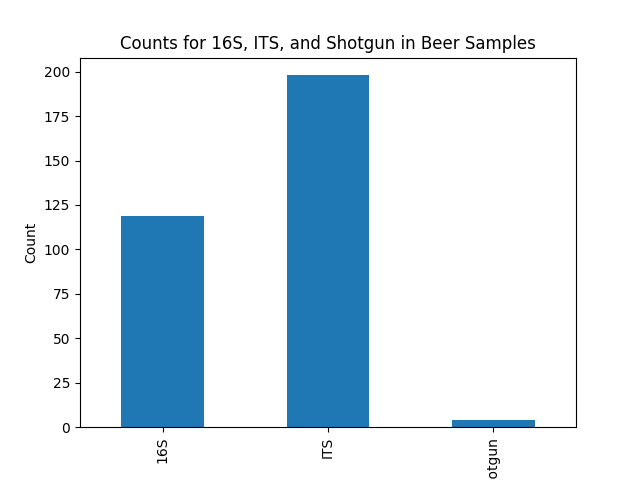
\includegraphics[scale=0.5]{images/overview/16S_ITS_Shotgun.png}
        \caption{Beer sample count}
        \label{fig:results:beer_sample_count}
    \end{figure}

    Overall, the BeerMicroDB database comprises a total of 119 samples analyzed via 16S rRNA gene sequencing, 198 samples examined using ITS sequencing, and a significantly smaller subset of just 4 samples studied using shotgun metagenomic sequencing (Figure \ref{fig:results:beer_sample_count}). It's clear that our current database is predominantly populated with data from metabarcoding methods, namely 16S and ITS sequencing.
    
    Despite the robustness and insights these methods offer, the relative scarcity of shotgun metagenomic data in our collection does present a limitation in terms of the depth and granularity of our microbial community analysis. We acknowledge this disparity in data types and emphasize the need to enhance the proportion of shotgun metagenomic data within BeerMicroDB. As such, we are hopeful that with the recommencement of the BeerDEcoded and Street Science Project, which help public citizens aware of bioinformatics by learning from sequencing to analyzing beer microbiome, we will be able to enrich our database with more shotgun metagenomic data, thus improving the breadth and depth of our analyses and leading to more nuanced insights into the beer microbiome.

\subsubsection{Fungal microbiome overview}

This section gives an overview of fungal microbiome results.

As shown in figure \ref{fig:methods:top10_beer_fungal}, the beer sample with the highest fungal species count was "Sesotho," which contained an impressive number of 70 distinct species. This was followed by "Rubi Marzen Lager" and "Extra Doppelbock Lager," hosting 51 and 46 species respectively. These beers exhibited significantly higher fungal biodiversity compared to others in the analysis. For instance, "Blond Beer (8.88\%)," "Chimay Red Cap," "Waldbier 2014 Wienerwald," "La Fourbe," "Valaisanne Amrich," and "La Montheysanne" exhibited species counts ranging from 7 to 21.

    \begin{figure}[H]
        \centering
        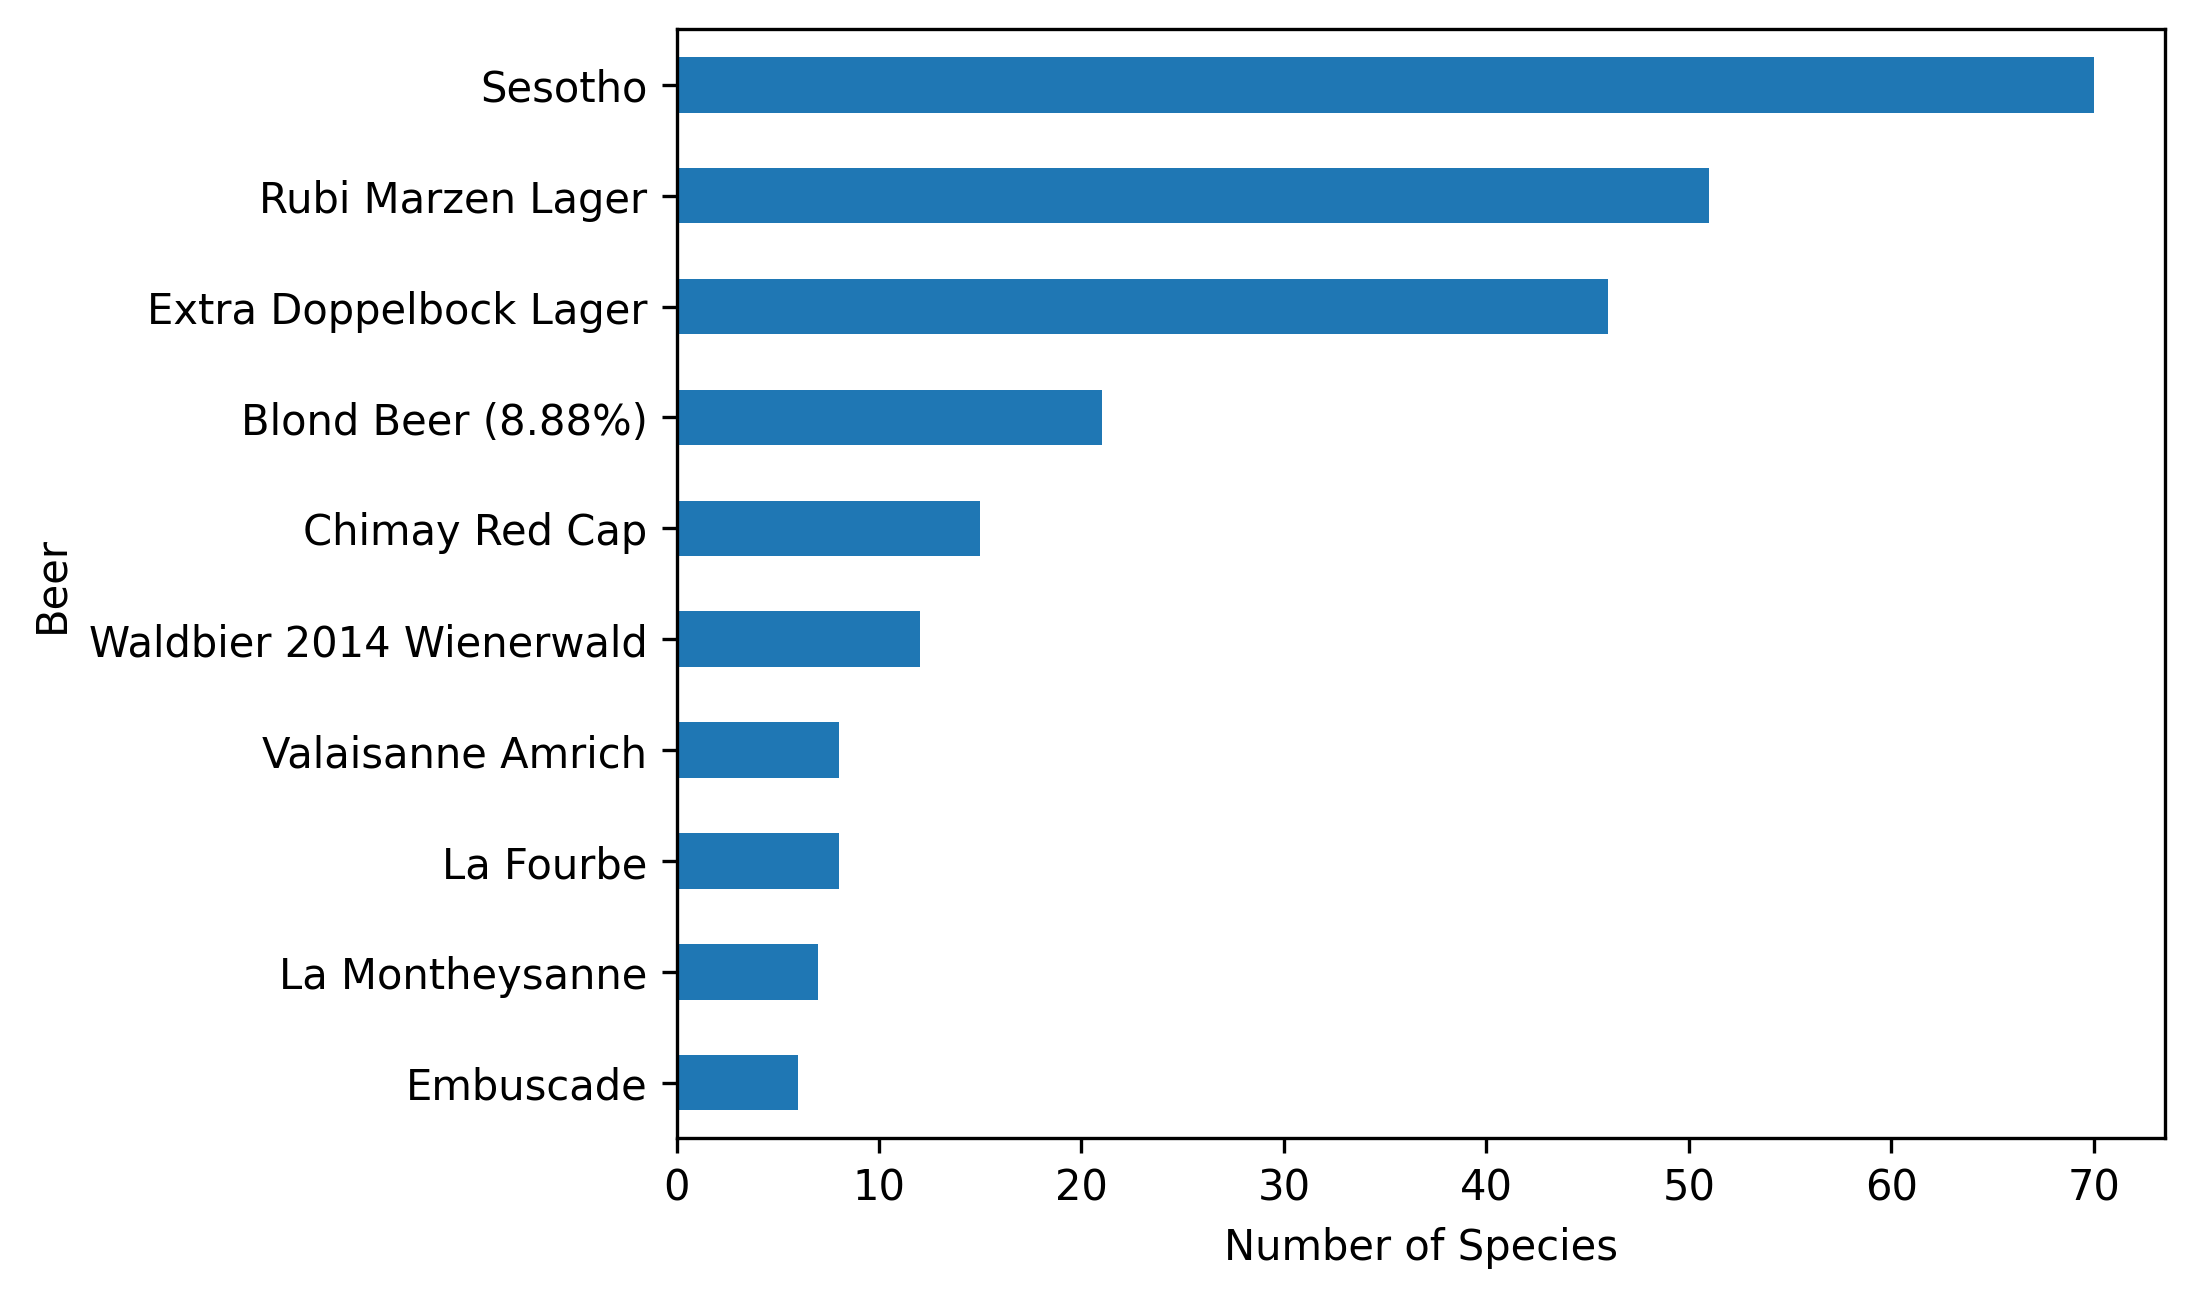
\includegraphics[scale=0.7]{images/overview/top10_beers_fungal.png}
        \caption{Top 10 Beers with the Highest Species Count}
        \small Among all beer types, Sesotho, which undergoes spontaneous fermentation, exhibits the highest count of fungal species.
        \label{fig:methods:top10_beer_fungal}
    \end{figure}
    
The data suggest that beer type and presumably the specific brewing process might significantly influence the diversity of fungal species in the final product. The top beers all have less regulated brewing processes and conditions.

The fungal species with the highest frequency of occurrence across the beer samples was \textit{Saccharomyces cerevisiae} identified in 126 instances (Figure \ref{fig:results:top10_species_fungal}). This is unsurprising, given that \textit{S. cerevisiae} is a commonly used yeast in the brewing industry due to its robust fermentation capabilities and its contribution to beer's distinctive flavor profiles.

    \begin{figure}[H]
        \centering
        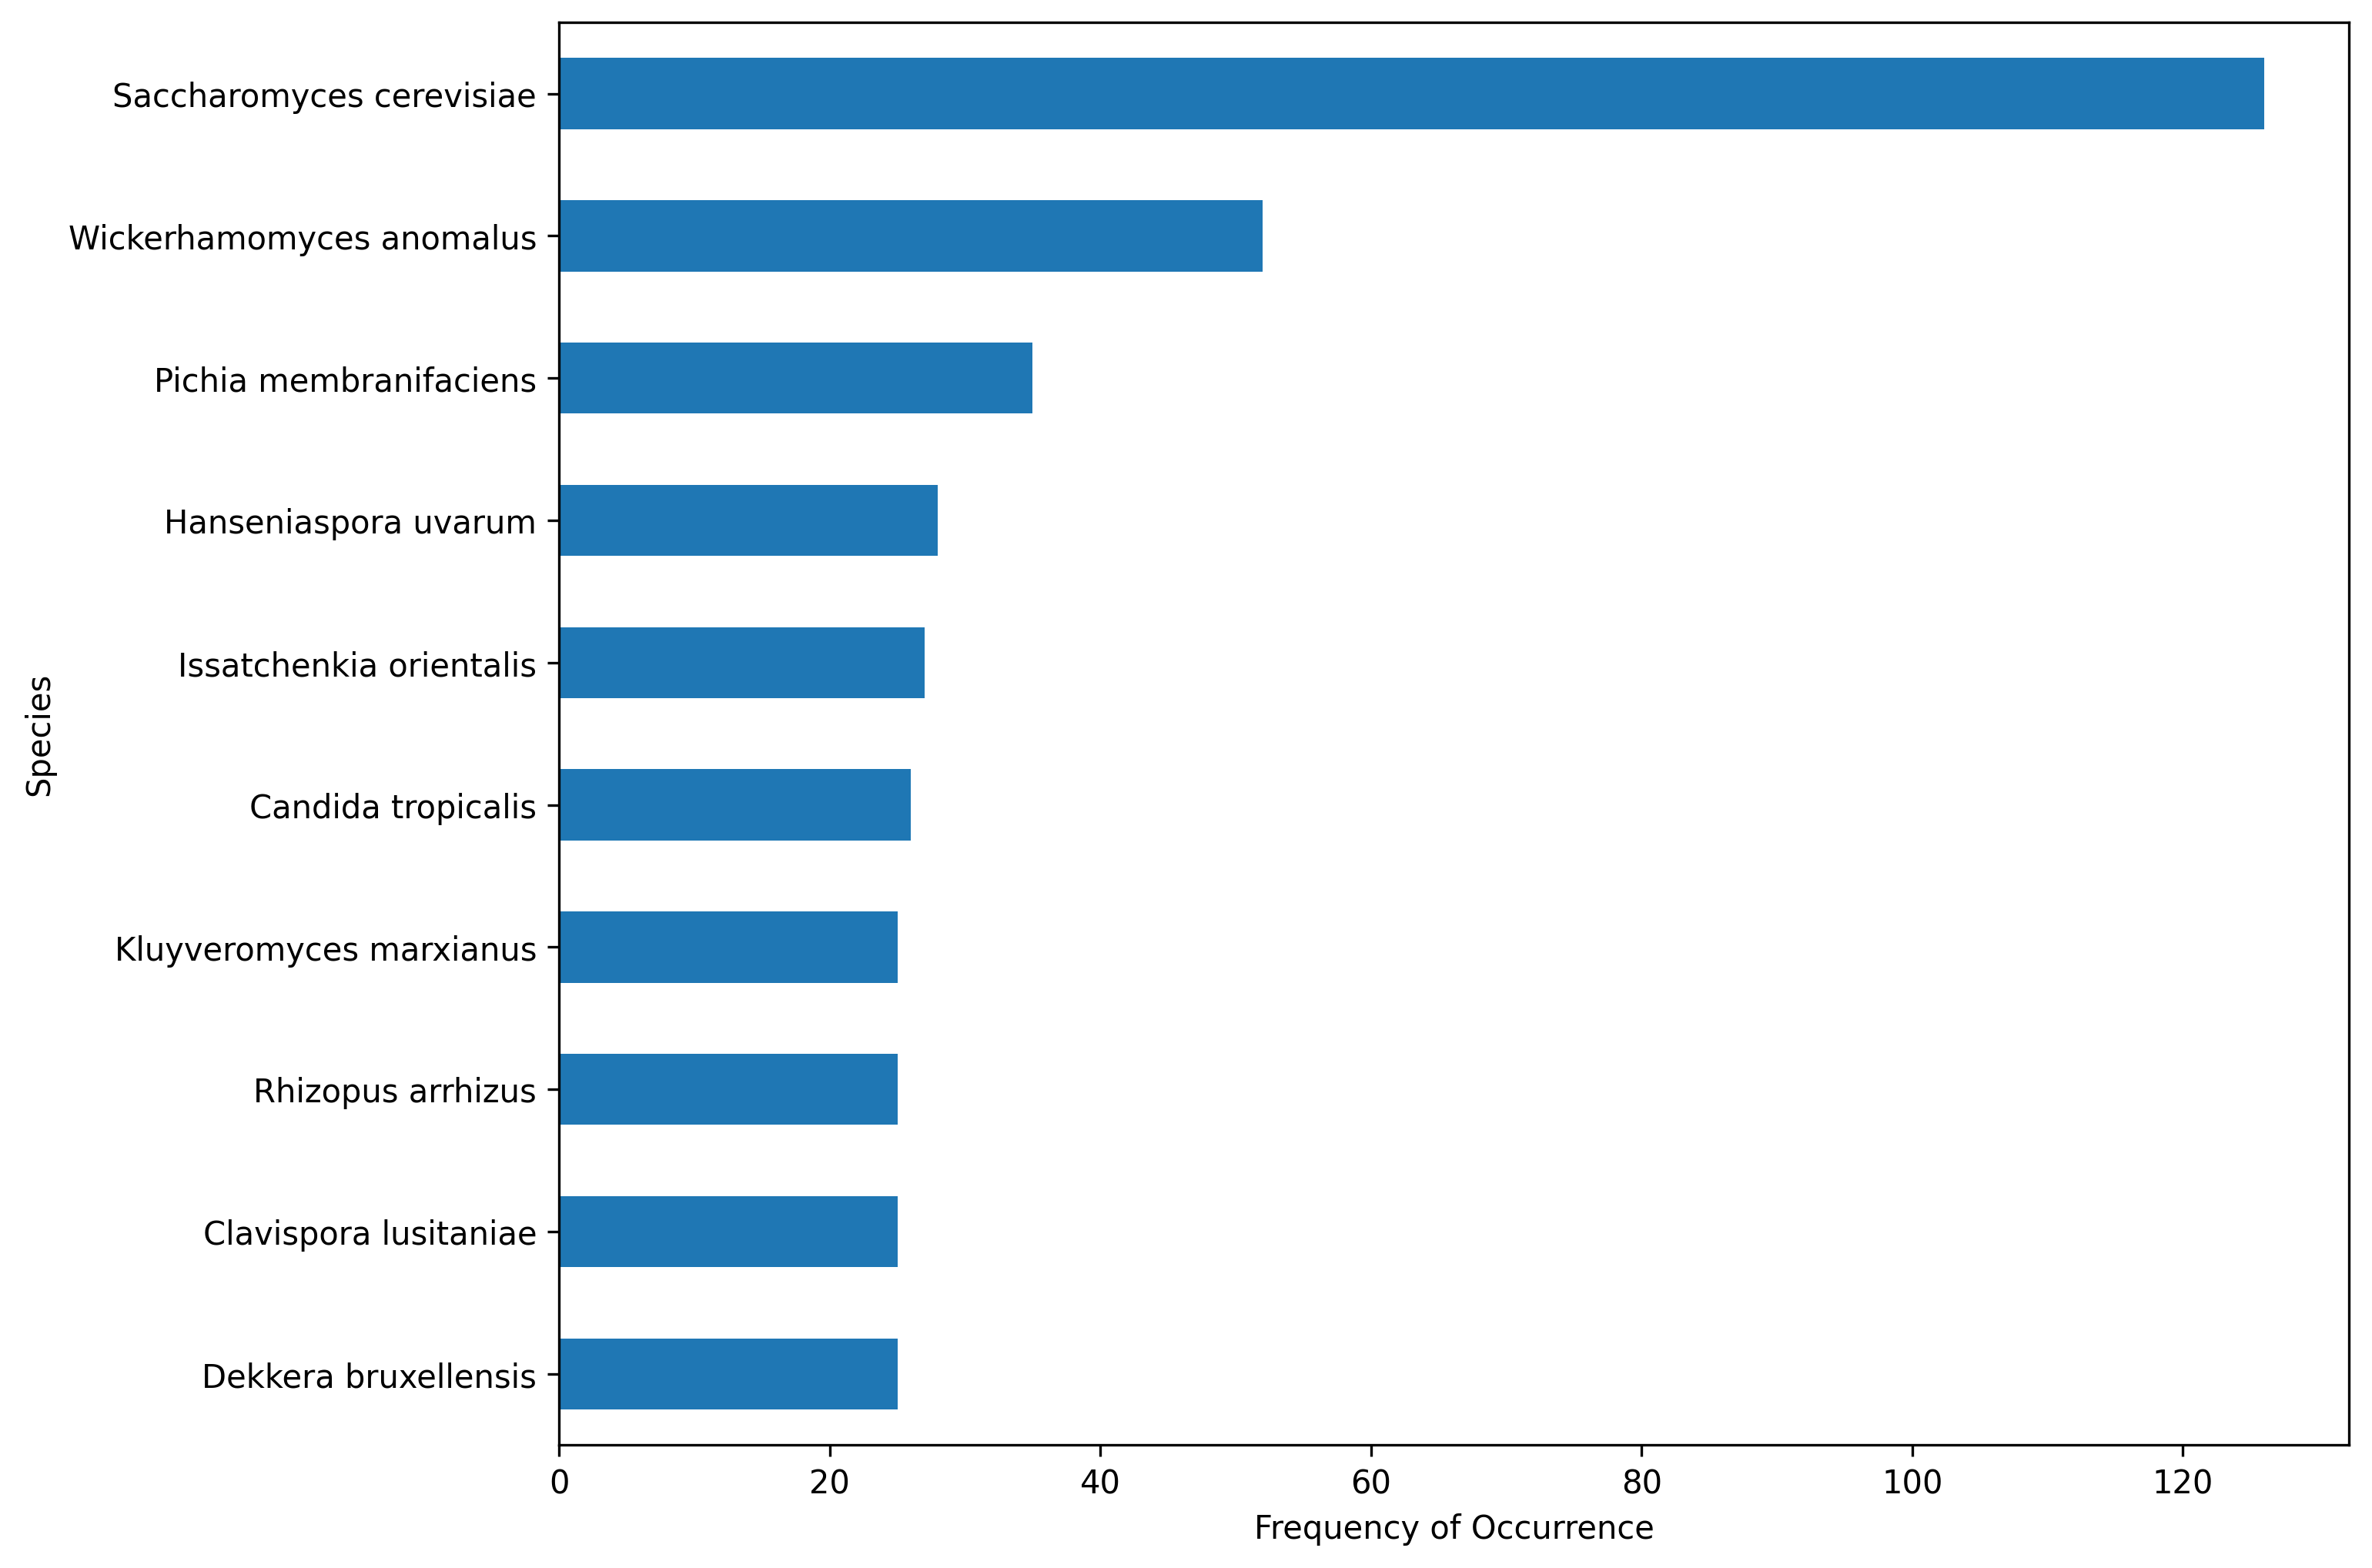
\includegraphics[scale=0.5]{images/overview/top10_species_fungal.png}
        \caption{Top 10 Species with the Highest Frequency of Occurrence}
        \small \textit{Saccharomyces cerevisiae} unequivocally emerges as the most prevalent species. It is closely followed by \textit{Wickerhamomyces anomalus}, which holds a slight advantage over other fungal species in the dataset.
        \label{fig:results:top10_species_fungal}
    \end{figure}
    
Other recurrent species include \textit{Wickerhamomyces anomalus} and \textit{Pichia membranifaciens} noted in 52 and 35 instances respectively, and a group of species including \textit{Hanseniaspora uvarum}, \textit{Issatchenkia orientalis}, \textit{Candida tropicalis}, \textit{Dekkera bruxellensis}, \textit{Clavispora lusitaniae}, \textit{Rhizopus arrhizus} and \textit{Kluyveromyces marxianus} each of which appeared 25-28 times.

These findings highlight the prevalence and importance of these species in the beer brewing ecosystem. It should be noted that while some of these species, such as \textit{D. bruxellensis} can potentially impart off-flavors to beer, others like \textit{K. marxianus} and \textit{W. anomalus} are known to have potentially beneficial effects on flavor and aroma complexity as shown before. Therefore, these species' presence and frequency could play a significant role in shaping the unique characteristics of the beers analyzed.
        


\subsubsection{Bacterial microbiome overview}

This section gives an overview of bacterial microbiome results from the 119 16S samples. The data revealed a diverse range of bacterial species associated with the beers, indicating the presence of complex microbial communities that potentially contribute to the unique flavors and characteristics of each brew. Two key aspects were explored: the top 10 beers with the highest species count and the top 10 species with the highest frequency of occurrence.

    \begin{figure}[H]
        \centering
        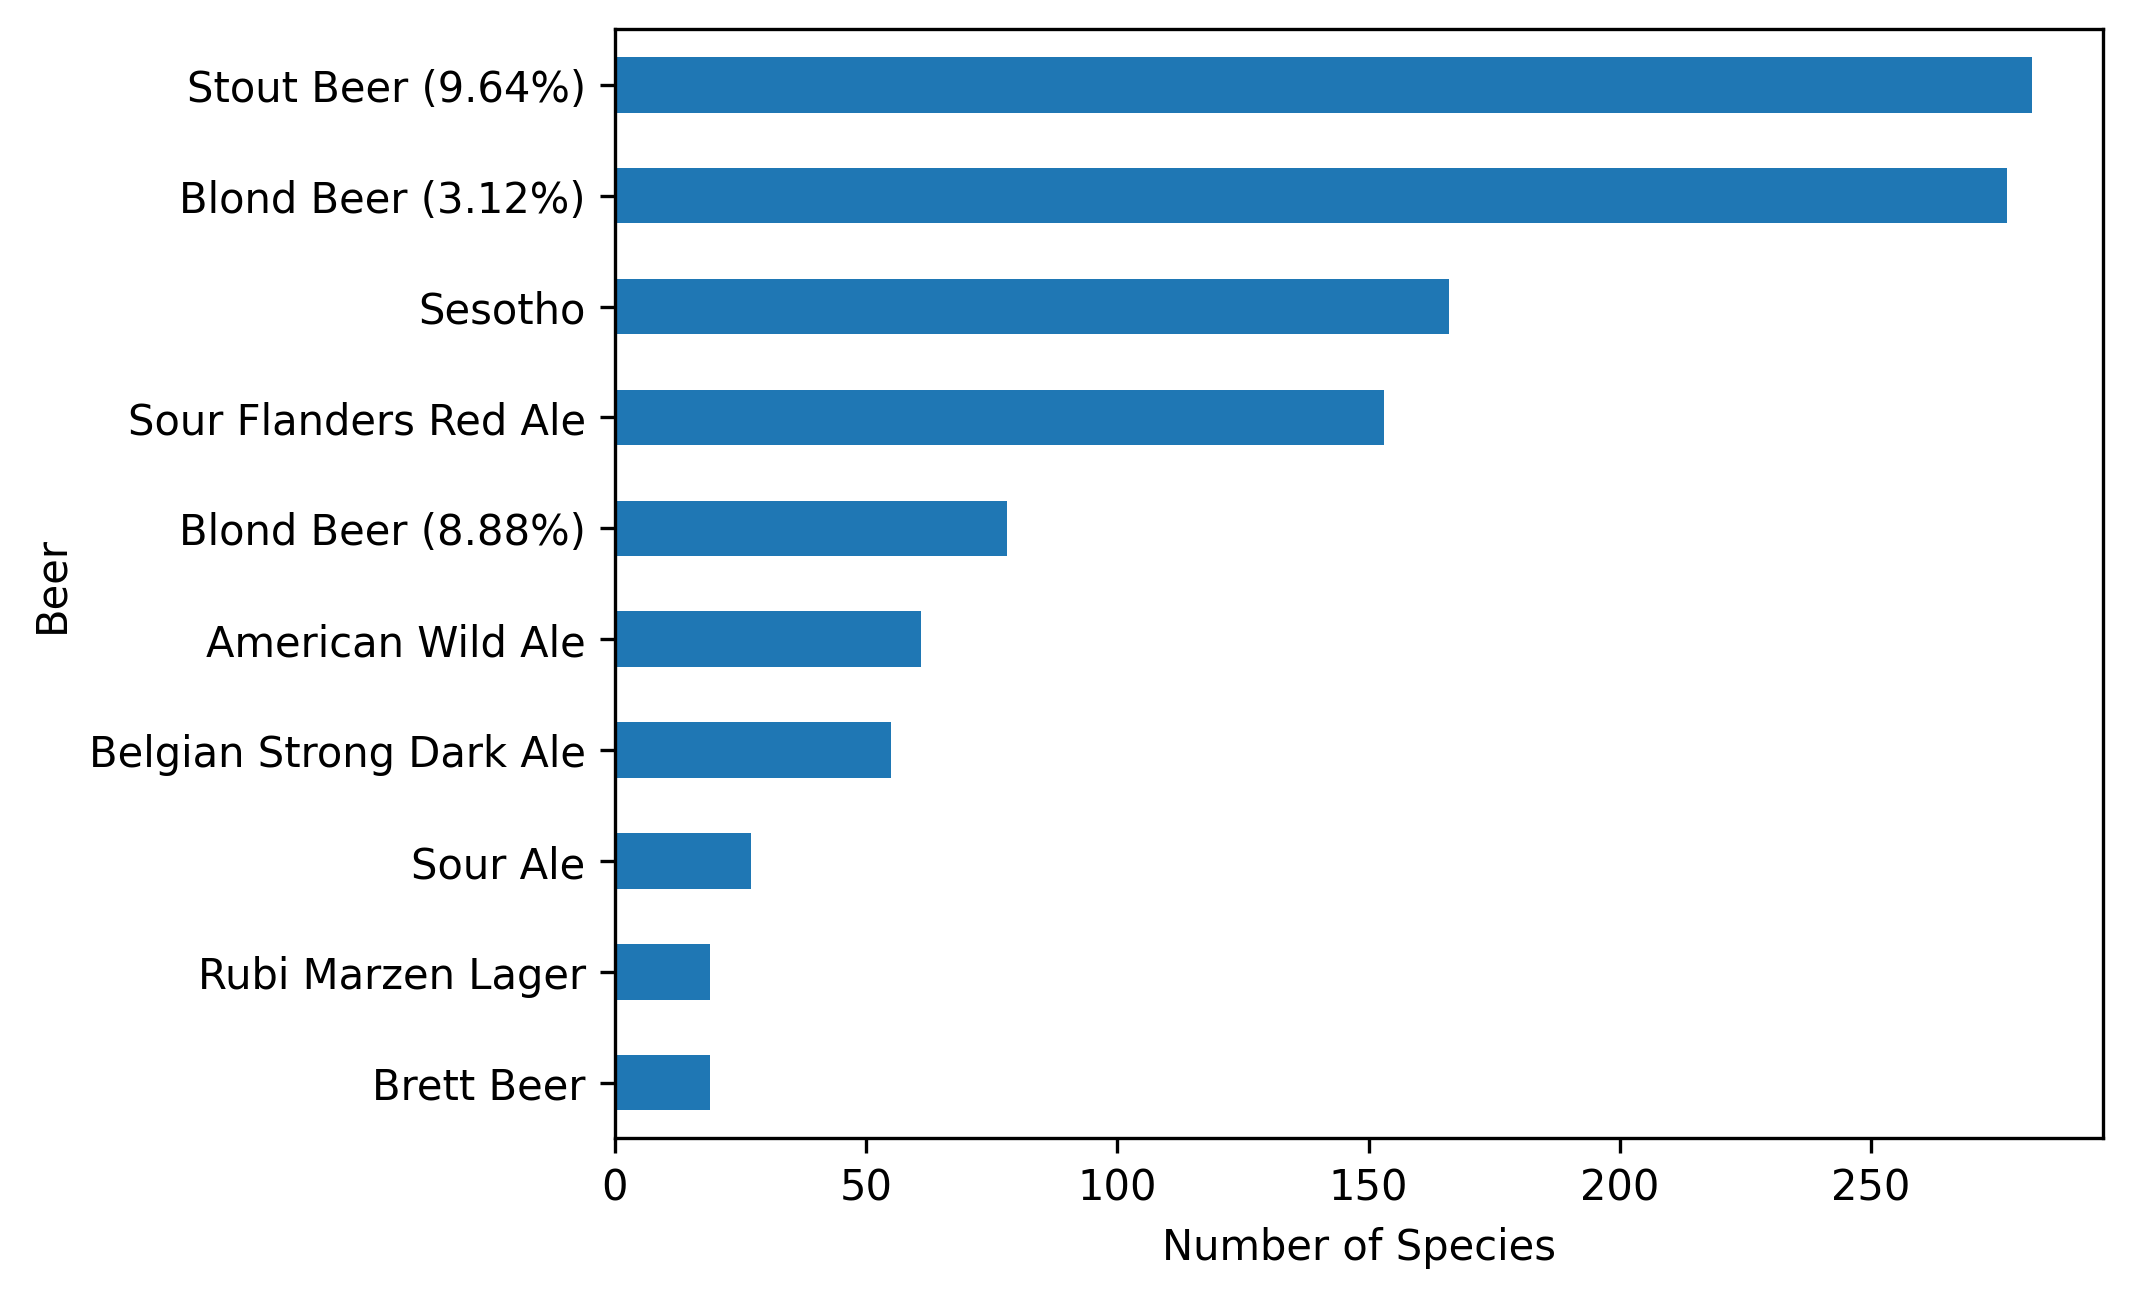
\includegraphics[scale=0.7]{images/overview/top10_beers_bac.png}
        \caption{Top 10 Beers with the Highest Species Count}
        \small The stout beer (9.64\%) and blond beer (3.12\%) lead in terms of bacterial species richness. They are closely followed by Sesotho and sour Flanders red ale in the subsequent rankings.
        \label{fig:results:top10_beer_bacterial}
    \end{figure}

The analysis of the bacterial microbiome in different types of beer unveils a complex and diverse bacterial composition. Notably, Stout Beer with a 9.64\% alcohol content exhibits the highest species count (282), followed closely by Blond Beer at two different alcohol percentages, 3.12\% (277 species) and 8.88\% (78 species) shown in the figure \ref{fig:results:top10_beer_bacterial}.

Interestingly, the presence of a beer called Sesotho, containing 166 species, indicates a potential regional influence on microbial diversity. Other notable inclusions are Sour Flanders Red Ale (153 species), American Wild Ale (61 species), Belgian Strong Dark Ale (55 species), Sour Ale (27 species), Brett Beer (19 species), and Rubi Marzen Lager (19 species).

The stour beer and blond beer went through a barrel aging process, this could be the reason why they have a high bacterial species count. And Sesotho which is spontaneously fermented in the wild environment, could be the reason why it is with high diversities. Overall, as we can see, the sour beer, ale has higher bacterial diversity.

    \begin{figure}[H]
        \centering
        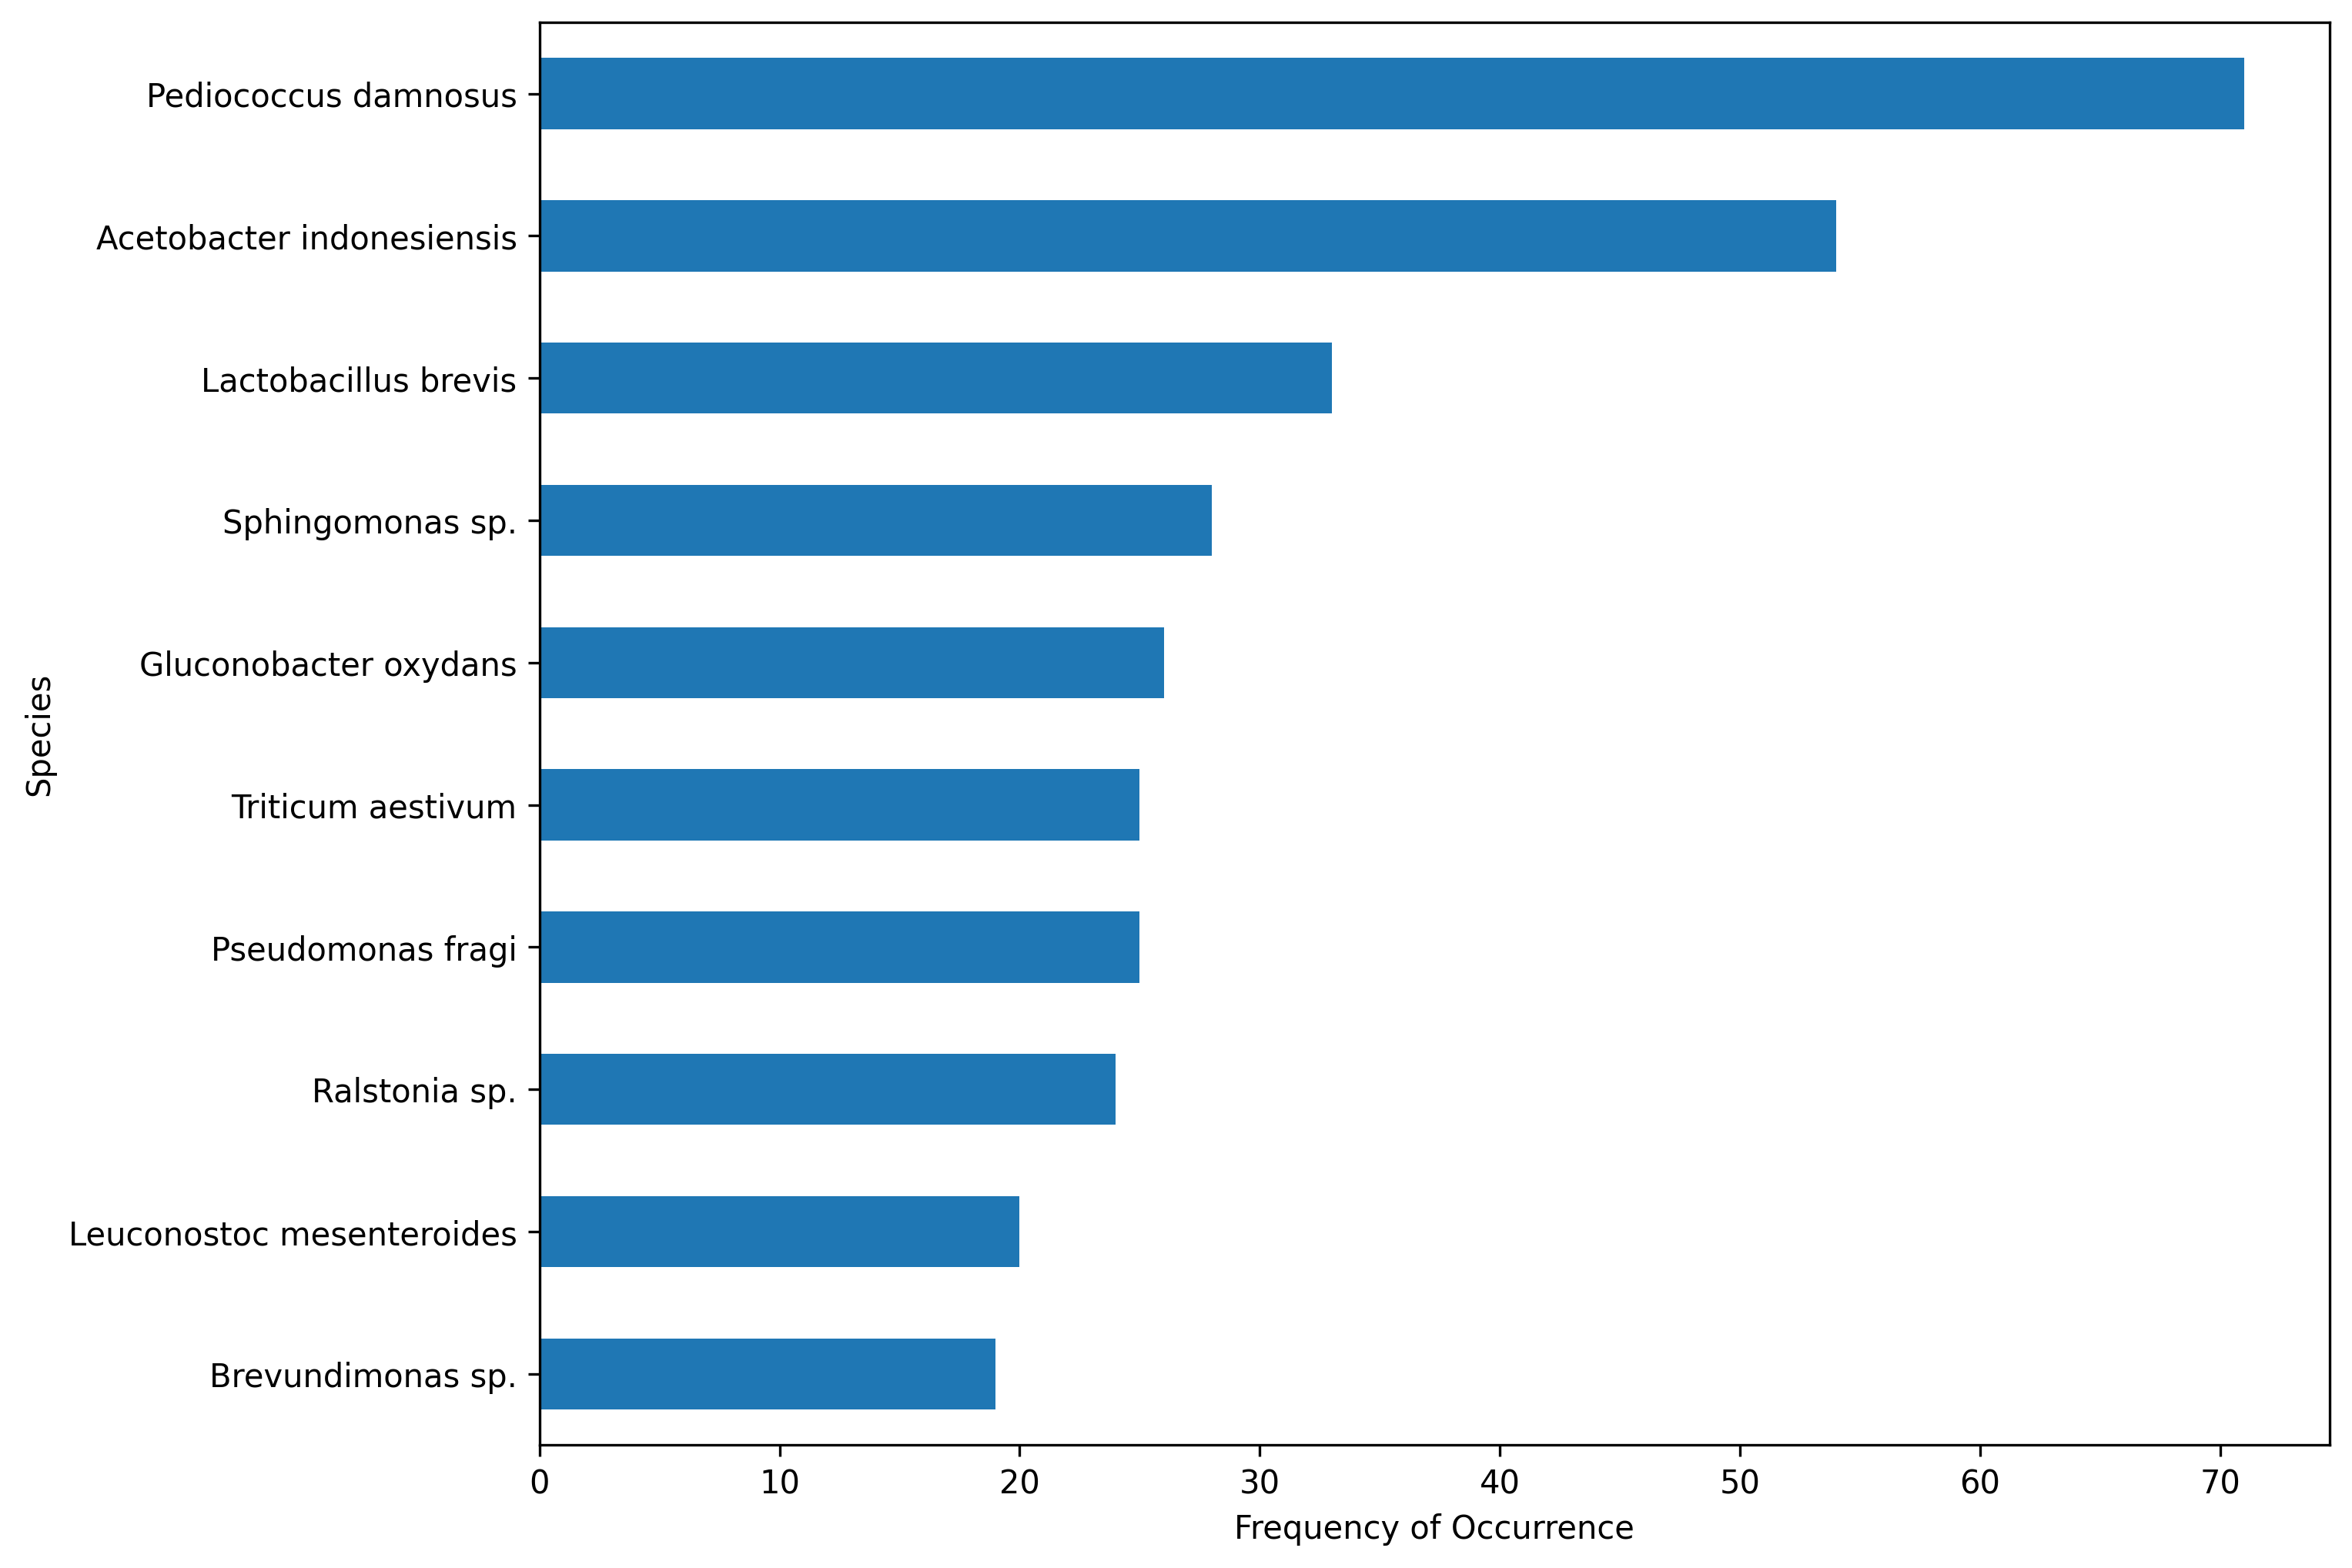
\includegraphics[scale=0.5]{images/overview/top10_species_bac.png}
        \caption{Top 10 Species with the Highest Frequency of Occurrence}
        \small The species \textit{Pediococcus damnosus} emerged as the most dominant, closely followed by \textit{Acetobacter indonesiensis}. Among the subsequent species observed, eight exhibited fewer differences in their frequency of occurrence.
        \label{fig:methods:top10_species_bac}
    \end{figure}
    
A close inspection of the top ten bacterial species, in terms of frequency of occurrence, highlights the significant presence of certain bacteria across different beer samples (Figure \ref{fig:methods:top10_species_bac}). The most prevalent species is \textit{Pediococcus damnosus}, found in 71 samples, followed by \textit{Acetobacter indonesiensis} (54), \textit{Lactobacillus brevis} (33), and \textit{Sphingomonas sp.} (28).

The presence of \textit{Gluconobacter oxydans} (26), \textit{Pseudomonas fragi} (25), \textit{Triticum aestivum} (25), \textit{Ralstonia sp.} (24), \textit{Leuconostoc mesenteroides} (20), and \textit{Brevundimonas sp.} (19) also suggests their common role in various beer types. These species are often involved in fermentation processes and may contribute to the unique flavors, aromas, and characteristics of the beer.

Furthermore, the occurrence of \textit{Triticum aestivum} might be indicative of wheat's role in certain beer formulations. The identification and characterization of these bacteria not only provide insights into the microbiological profile of different beers but also raise potential considerations in quality control, flavor development, and potential health aspects.

In conclusion, these findings serve as an essential resource for understanding the intricate bacterial ecology within various beer types, contributing to ongoing research in brewing science, quality assurance, and sensory analysis. Further studies may elucidate the specific roles and interactions of these microbial communities in shaping the attributes of the diverse world of beer.
     